\documentclass[master=cws,masteroption=gs]{kulemt}

% bijkomende packages

\usepackage[dutch]{babel}

\usepackage[all,color]{xy}
\xyoption{all}

\usepackage{subcaption}

\usepackage{mathtools}

\usepackage{xspace}

\usepackage{minted}

\usepackage{algorithm}
\usepackage{algpseudocode}

\usepackage{bm}

% enkele persoonlijke commands

\newcommand{\TODO}{\textbf{\color{red}TODO}}


%!TEX root=masterproef.tex

\setup{
  title={Verlagen van de impact van inbraakdetectie
         in draadloze sensornetwerken
         door middel van een domeinspecifieke taal
         en codegeneratietechnieken},
  author={Christophe Van Ginneken},
  promotor={Prof.\,dr.\,ir.\ Wouter Joosen \and Prof.\,dr.\,ir.\ Christophe Huygens},
  assessor={Dr.\ Benjamin Negrevergne \and Dr.\ Nelson Matthys},
  assistant={Drs.\,ir.\ Jef Maerien}
}

\setup{
  filingcard,
  translatedtitle={Lowering the Impact of Intrusion Detection
                   in Wireless Sensor Networks
                   using a Domain Specific Language
                   \& Code Generation Techniques},
  udc=681.3,
  shortabstract={
Draadloze sensornetwerken treden met rasse schreden onze persoonlijke
levenssfeer binnen. Beveiliging tegen inbraken moet garanties bieden dat deze
vooruitgang zelf geen bedreiging wordt. Preventie is de eerste stap, maar niet
alle inbraken kunnen vermeden worden. Soms moeten we genoegen nemen met het
detecteren ervan om ons in de toekomst er beter tegen te wapenen. Het
introduceren van inbraakdetectie in draadloze sensornetwerken resulteert al
snel in een gevecht om middelen: een draadloze sensorknoop beschikt over een
beperkte autonomie en moet zijn energie optimaal benutten. Inbraakbeveiliging
vraagt veel van de beschikbare middelen en hypothekeert daarmee de kans om
opgenomen te worden in het uiteindelijke ontwerp van elke nieuwe draadloze
sensorknoop. Indien het probleem niet kan vermeden worden, moeten we trachten
het draaglijker te maken. De introductie van inbraakdetectie heeft een impact
op verschillende vlakken. Deze masterproef wil zowel de druk op de middelen van
de sensorknopen verlichten als de bijkomende economische druk op de
ontwikkeling reduceren. Om dit te realiseren, wordt een domeinspecifieke taal
voorgesteld die onderzoekers in staat stelt om algoritmen voor inbraakdetectie
op een formele en platformonafhankelijke manier te defini\"eren. Deze eerste
stap ontslaat ontwikkelaars van nieuwe sensornetwerken van de taak om
onderzoeksliteratuur te doorworstelen en algoritmen uit deze teksten te puren.
Een formele beschrijving laat verder toe om deze algoritmen op geautomatiseerde
wijze te benaderen. Zo wordt het mogelijk om door middel van codegeneratie de
algoritmen automatisch om te zetten in platformspecifieke programmacode, z\'o
georganiseerd dat de middelen van de sensorknoop zo optimaal mogelijk benut
worden. De initi\"ele testen met een prototype codegenerator zijn veelbelovend.
Ze bevestigen de intu\"itie dat een goede organisatie van verschillende
detectiealgoritmen kan leiden tot een beter gebruik van de middelen van een
sensorknoop \'en dat dit volledig geautomatiseerd kan gebeuren. Dankzij het
vrijwaren van de middelen van de sensorknoop en het reduceren van de
economische kost, wordt het zo mogelijk om meer inbraakpogingen te detecteren.
Zowel de domeinspecifieke taal als de codegenerator bieden opportuniteiten tot
verder onderzoek. Testen met detectiealgoritmen en platformen moeten op grotere
schaal uitgewerkt worden. De realisatie van een ecosysteem rond de
geformaliseerde detectiealgoritmen is een andere belangrijke richting die
nagestreefd moet worden en waar vooral het onderzoeksdomein baat bij heeft.
} }


%\setup{coverpageonly}
\setup{font=lm}

\begin{document}

% to avoid syntax error highlighting - e.g. foo's not js ;-)
\expandafter\def\csname PY@tok@err\endcsname{}

%!TEX root=masterproef.tex

\begin{preface}

Het is niet iedereen gegeven om op 40 jarige leeftijd een masterproef te mogen,
of eerder kunnen, maken. De keuze om opnieuw te gaan studeren maak je niet
alleen en vraagt van veel mensen een bijzondere inspanning. Familie en
vrienden, maar ook professoren en assistenten worden plots uit hun vertrouwde
omgeving weggerukt en worden geconfronteerd met een ongewone situatie.

Net zoals snel zal blijken, is deze masterproef het resultaat van veel meer dan
de afgelopen drie jaren van hernieuwde studie aan de universiteit van Leuven.
Oude en nieuwe ervaringen gaan hand in hand en hebben geleid tot vragen en
antwoorden die samen groter zijn dan de som van de afzonderlijke delen.

Dat ik deze masterproef heb kunnen realiseren met de hulp van een ongelooflijk
team is slechts het topje van de ijsberg. Dat de mensen in dit team ook nog
eens een band hebben met het verleden typeert meer dan eens de ondertoon van
deze masterproef.

Professor dr. ir. Wouter Joosen en prof. dr. ir. Christophe Huygens beseffen
het misschien niet ten volle, maar staan eens te meer aan de bakermat van mijn
toekomst. Hun passie en gedrevenheid zijn opnieuw een ongelooflijke bron van
inspiratie geweest om dit moeilijke onderwerp aan te pakken en het tot een goed
einde te brengen.

Ofschoon de ongewone situatie soms zorgde voor spanningen, was Jef Maerien
tevens de enige juiste begeleider, die mijn vlot op deze woelige rivier
dikwijls met een klein manoeuvre op koers wist te houden. Sorry voor mijn soms
arrogante attitude en bedankt voor het behouden vertrouwen. Jouw kritische
opmerkingen hebben mijn meer dan eens op de tippen van mijn tenen gehouden en
hebben op verschillende vlakken geleid tot betere resultaten.

TODO: assessoren

Maar ondanks de ongelooflijke steun van dit team, was deze masterproef nooit
gelukt zonder een nog groter team op het thuisfront. Drie jaar terug gaan
studeren overstijgt een klassieke dagtaak en legt een veel grotere dan verwacht
druk op een gezin. Kristien, mijn echtgenote, heeft elke seconde van de
afgelopen drie jaar, elke druppel zweet en tranen mee door gemaakt, ouders en
schoonouders hebben op de meest onmogelijke momenten ingesprongen om mij tijd
en ruimte te geven om dit huzarenstukje te realiseren. Meer dan eens moesten we
beroep doen op vrienden en buren om allerhande elementaire karwijen in mijn
plaats op te lossen. Het is hallucinant en hartverwarmend om te ervaren hoe
zoveel mensen meegeleefd hebben met mij.

Tot slot zijn er nog twee mensen die echt een hele dikke knuffel verdienen. Van
iedereen begrijpen zij misschien het minst wat papa gedaan heeft de afgelopen
jaren en waarom er zo weinig tijd voor hen overbleef. Eline en Arjen, mijn
lieve schatten, bedankt dat jullie soms zo begripvol waren en me dikwijls
opnieuw moed hebben gegeven om toch door te gaan.

\bigskip

Bedankt!

\end{preface}


\tableofcontents*

\begin{abstract}

In dit \texttt{abstract} environment wordt een al dan niet uitgebreide
samenvatting van het werk gegeven. De bedoeling is wel dat dit tot 1 bladzijde
beperkt blijft.

\end{abstract}

%!TEX root=masterproef.tex


\listoffigures
\listoftables
\listoflistings
\addcontentsline{toc}{chapter}{Lijst van codevoorbeelden}

%!TEX root=masterproef.tex

\chapter{Lijst van afkortingen}

\TODO aanvullen

\begin{flushleft}
  \renewcommand{\arraystretch}{1.1}
  \begin{tabularx}{\textwidth}{@{}p{24mm}X@{}}

AAA       &  Authentication Authorisation Accounting \\
AST       &  Abstract Syntax Tree \\
CDA       &  Concealed Data Aggregation \\
CIA       &  Confidentiality Integrity Availability \\
CM        &  Code Model \\
DoS       &  Denial of Service \\
GHz       &  Giga Hertz \\
IDP       &  Intrusion Detection Problem \\
IDS       &  Intrusion Detection System \\
LR-WPAN   &  Low-Rate Wireless Personal Area Networks \\
MAC       &  Media Access Control \\
MANET     &  Mobile and Adhoc NETwork \\
MCL       &  M-Core Control Language \\
MHz       &  Mega Hertz \\
OTAP      &  Over The Air Programming \\
PAN       &  Personal Area Network \\
PDP       &  Policy Decision Point \\
PEP       &  Policy Enforcement Point \\
PIP       &  Policy Information Point \\
SM        &  Semantic Model \\
SoC       &  System on Chip \\
WSN       &  Wireless Sensor Network \\
\mcu      &  microcontroller \\

  \end{tabularx}
\end{flushleft}


\mainmatter

%!TEX root=masterproef.tex

\chapter{Inleiding}
\label{inleiding}

Ze hebben de voorpagina van de krant dan misschien nog niet gehaald, de opmars
van draadloze sensornetwerken (DSN) in ons dagelijks leven is niet meer te
stoppen. Na de revolutie van de persoonlijke computer, de smartphone en het
tablet vinden nu onafhankelijke, minuscule computers hun weg naar allerlei
alledaagse dingen en plaatsen in ons leven. Deze netwerken kunnen met hun
sensoren de kleinste wijzigingen in hun omgeving optekenen. Via een draadloos
netwerk staan de sensoren in verbinding met elkaar en de buitenwereld. Zo
leveren ze hun informatie af, waardoor wij op elk moment precies weten hoe warm
het in elke kamer van ons huis is of welke groenten nog in de koelkast liggen.
Het lijkt nog science fictie, maar deze toekomst is heel wat dichterbij dan we
vermoeden.

Om deze technologie te omarmen en ons leven verder in te richten met deze
ondersteunende hulp, moeten we ons er van vergewissen dat deze technologie
betrouwbaar en veilig is. Als enkele sensoren in ons huis slechts een kleine
stap met weinig potenti\"ele, problematische gevolgen lijkt, moeten we ons toch
bezinnen en beseffen dat al deze kleine computers zeer interessante
inbraakmogelijkheden bieden aan anderen met minder positieve bedoelingen.

Misschien wil de concurrent van de producent van onze yoghurt zijn collega wel
in diskrediet brengen door er voor te zorgen dat onze slimme koelkast het
nalaat ons te verwittigen dat de yoghurt vervallen is. Misschien vindt de
gasleverancier het wel leuk om, wanneer we niet thuis zijn, de thermostaat een
graadje hoger te zetten.

De mogelijkheden van draadloze sensornetwerken lijken eindeloos en ze kunnen de
kwaliteit van ons leven ingrijpend veranderen. Ze mogen echter geen bijkomende
bedreiging introduceren. In deze masterproef duiken we in de wereld van
draadloze sensornetwerken en willen we nagaan of en hoe we deze kunnen voorzien
van bescherming tegen minder goede bedoelingen.

Sectie \ref{section:wsn} introduceert draadloze sensornetwerken. Hoe zijn ze
opgebouwd? Wat zijn de mogelijkheden en beperkingen? 

Sectie \ref{section:beveiligen} legt de nadruk op beveiliging: Wat zijn de
gevaren? Hoe kunnen deze vastgesteld worden? Hoe kunnen sensorknopen beschermd
worden?

Sectie \ref{section:probleem} brengt beide aspecten samen en vat de
probleemstelling samen.

Sectie \ref{section:doelstelling} legt tot slot kort de doelstelling van deze
masterproef uit.

\section{Draadloze sensornetwerken}
\label{section:wsn}

Sinds de late jaren '90 zijn draadloze sensornetwerken een bron geweest voor
een overvloed aan onderzoek. Binnen en buiten universiteiten werden deze
netwerken ingezet voor allerhande toepassingen: van het opvolgen van
microklimaten bij het telen van gewassen \citep{baggio2005wireless} tot het
vastleggen van vulkanische activiteit \citep{werner2005monitoring} en het
opvolgen van overstromingsgebieden \citep{hughes2006gridstix}.

Wat moeten we ons eigenlijk voorstellen bij een draadloos sensornetwerk? We
bekijken kort de sensorknopen, waarmee het netwerk wordt opgebouwd. Vervolgens
belichten we het draadloze netwerk dat de knopen in staat stelt om met elkaar
en met de buitenwereld te communiceren.

\subsection{Sensorknopen}

Sensorknopen zijn in essentie zeer eenvoudige computers. Ze worden typisch
opgebouwd rond een microcontroller (\mcu). Dit is een digitaal ontwerp dat
zowel een processor als geheugen en invoer- en uitvoerkanalen bevat op \'e\'en
ge\"integreerde schakeling. Ze worden daarom ook wel \emph{systeem-op-een-chip}
(\emph{System-on-Chip}) (SoC) genoemd. Figuur \ref{fig:motes} toont enkele
typische sensorknopen.

\begin{figure}[ht]
\centering
\begin{subfigure}{.24\textwidth}
  \centering
  \includegraphics[width=.9\linewidth]{./resources/mica2.jpg}
  \caption{Mica2}
  \label{fig:mica2}
\end{subfigure}
\begin{subfigure}{.24\textwidth}
  \centering
  \includegraphics[width=.9\linewidth]{./resources/dot.png}
  \caption{Dot}
  \label{fig:dot}
\end{subfigure}
\begin{subfigure}{.24\textwidth}
  \centering
  \includegraphics[width=.9\linewidth]{./resources/telos.jpg}
  \caption{Telos}
  \label{fig:telos}
\end{subfigure}
\begin{subfigure}{.24\textwidth}
  \centering
  \includegraphics[width=.9\linewidth]{./resources/raven.jpg}
  \caption{AVRraven}
  \label{fig:raven}
\end{subfigure}
\caption{Voorbeelden van sensorknopen}
\label{fig:motes}
\end{figure}

Naast de \mcu heeft een typische sensorknoop tevens een draadloze radio. Je kan
dit vergelijken met de Wi-Fi verbinding die je tegenwoordig in de meeste
computers of smartphones vindt. Voor sensorknopen wordt echter meestal
geopteerd voor een draadloze radio die een minimum aan energie probeert te
verbruiken. Verschillende nieuwe draadloze netwerkstandaarden zijn de laatste
jaren op de voorgrond getreden. De bekendste zijn 6LoWPAN \citep{rfc:6282} en
ZigBee \citep{alliance2012zigbee}. In de volgende paragrafen bekijken we ZigBee
van naderbij; enerzijds omwille van de toepassing in deze masterproef, maar ook
omwille van de voorbeeldfunctie die het kan aannemen voor deze groep van
draadloze standaarden.

\subsection{ZigBee}
\label{subsection:zigbee}

ZigBee zelf is een laag bovenop de netwerklaag gekend als IEEE 802.15.4
\citep{ieee2009802.15.4}. Deze voorziet standaarden op vlak van energiegebruik,
adressering, foutcorrectie, vormgeving van berichten\dots en vormt zo de
fundamenten voor zgn. \emph{low-rate wireless personal area networks}
(LR-WPAN). ZigBee voegt hieraan nog drie belangrijke eigenschappen toe:
routering, ad-hoc netwerkcreatie en zelfherstellende maasnetwerken (\emph{mesh
networks}) \citep{oreilly2010buildingwsn}.

Een ZigBee-netwerk wordt opgebouwd door knopen die elk \'e\'en van drie
verschillende functies kunnen innemen: co\"ordinator, router of eindknoop.

\begin{description}

  \item[Co\"ordinator] Elk netwerk heeft \'e\'en \emph{co\"ordinator}. Deze
  knoop is verantwoordelijk voor het samenbrengen van het netwerk en definieert
  de eigenschappen, bv. met betrekking tot de beveiliging.

  \item[Router] Een \emph{router} stelt andere knopen in staat om met elkaar te
  communiceren. Deze knopen zijn daarom meestal voorzien van een permanente
  stroomvoorziening, omdat ze zich in tegenstelling tot \emph{eindknopen},
  wegens hun communicatieondersteunende rol, niet in een slaapstand kunnen
  zetten.

  \item[Eindkknoop] \emph{Eindknopen}, tot slot, kunnen zich louter verbinden
  met een netwerk, er berichten via versturen en berichten voor zichzelf
  ontvangen. Het is niet de bedoeling om berichten van andere knopen voor
  andere knopen door te sturen. Typisch trachten ze ook hun energieverbruik te
  minimaliseren door hun draadloze radio zoveel mogelijk uit te schakelen.
  Hierdoor worden ze op dat moment onbereikbaar. Het is dankzij \emph{routers},
  die berichten voor de \emph{eindknopen} tijdelijk opslaan, dat ze toch
  berichten kunnen ontvangen.

\end{description}

\subsection{Netwerktopologie en -adressen}
\label{subsection:topologie}

Met knopen kunnen verschillende netwerktopologie\"en gebouwd worden. Figuur
\ref{fig:topologie} geeft een overzicht van de mogelijkheden.

\begin{description}

  \item[Paar] In zijn eenvoudigste vorm bestaat een netwerk uit een
  co\"ordinator en een eindknoop. Deze minimalistische vorm is slechts een
  theoretische mogelijkheid ter volledigheid van de mogelijkheden.
  
  \item[Ster] Wanneer meerdere eindknopen verbonden zijn met dezelfde
  co\"ordinator, vormen zij een stertopologie. Alle communicatie verloopt via
  de centrale co\"ordinator.
  
  \item[Maasnetwerk] In een maasnetwerk worden routers ingeschakeld om
  communicatie via verschillende wegen mogelijk te maken. Eindknopen zijn
  verbonden met deze routers of met de co\"ordinator. Routers en co\"ordinator
  kunnen berichten ontvangen van eindknopen en deze versturen naar andere
  eindknopen, al dan niet via andere routers.
  
  \item[Clusterboom] Een speciale vorm van een maasnetwerk is een clusterboom.
  Hierbij vormen groepen van eindknopen en een router een cluster. De router is
  verbonden met de co\"ordinator, eventueel opnieuw via andere routers, en zo
  wordt een boomstructuur gevormd. De routers die de clusters van eindknopen
  realiseren worden ook clusterhoofden genoemd.
  
\end{description}

\begin{figure}[ht]
  \centering
  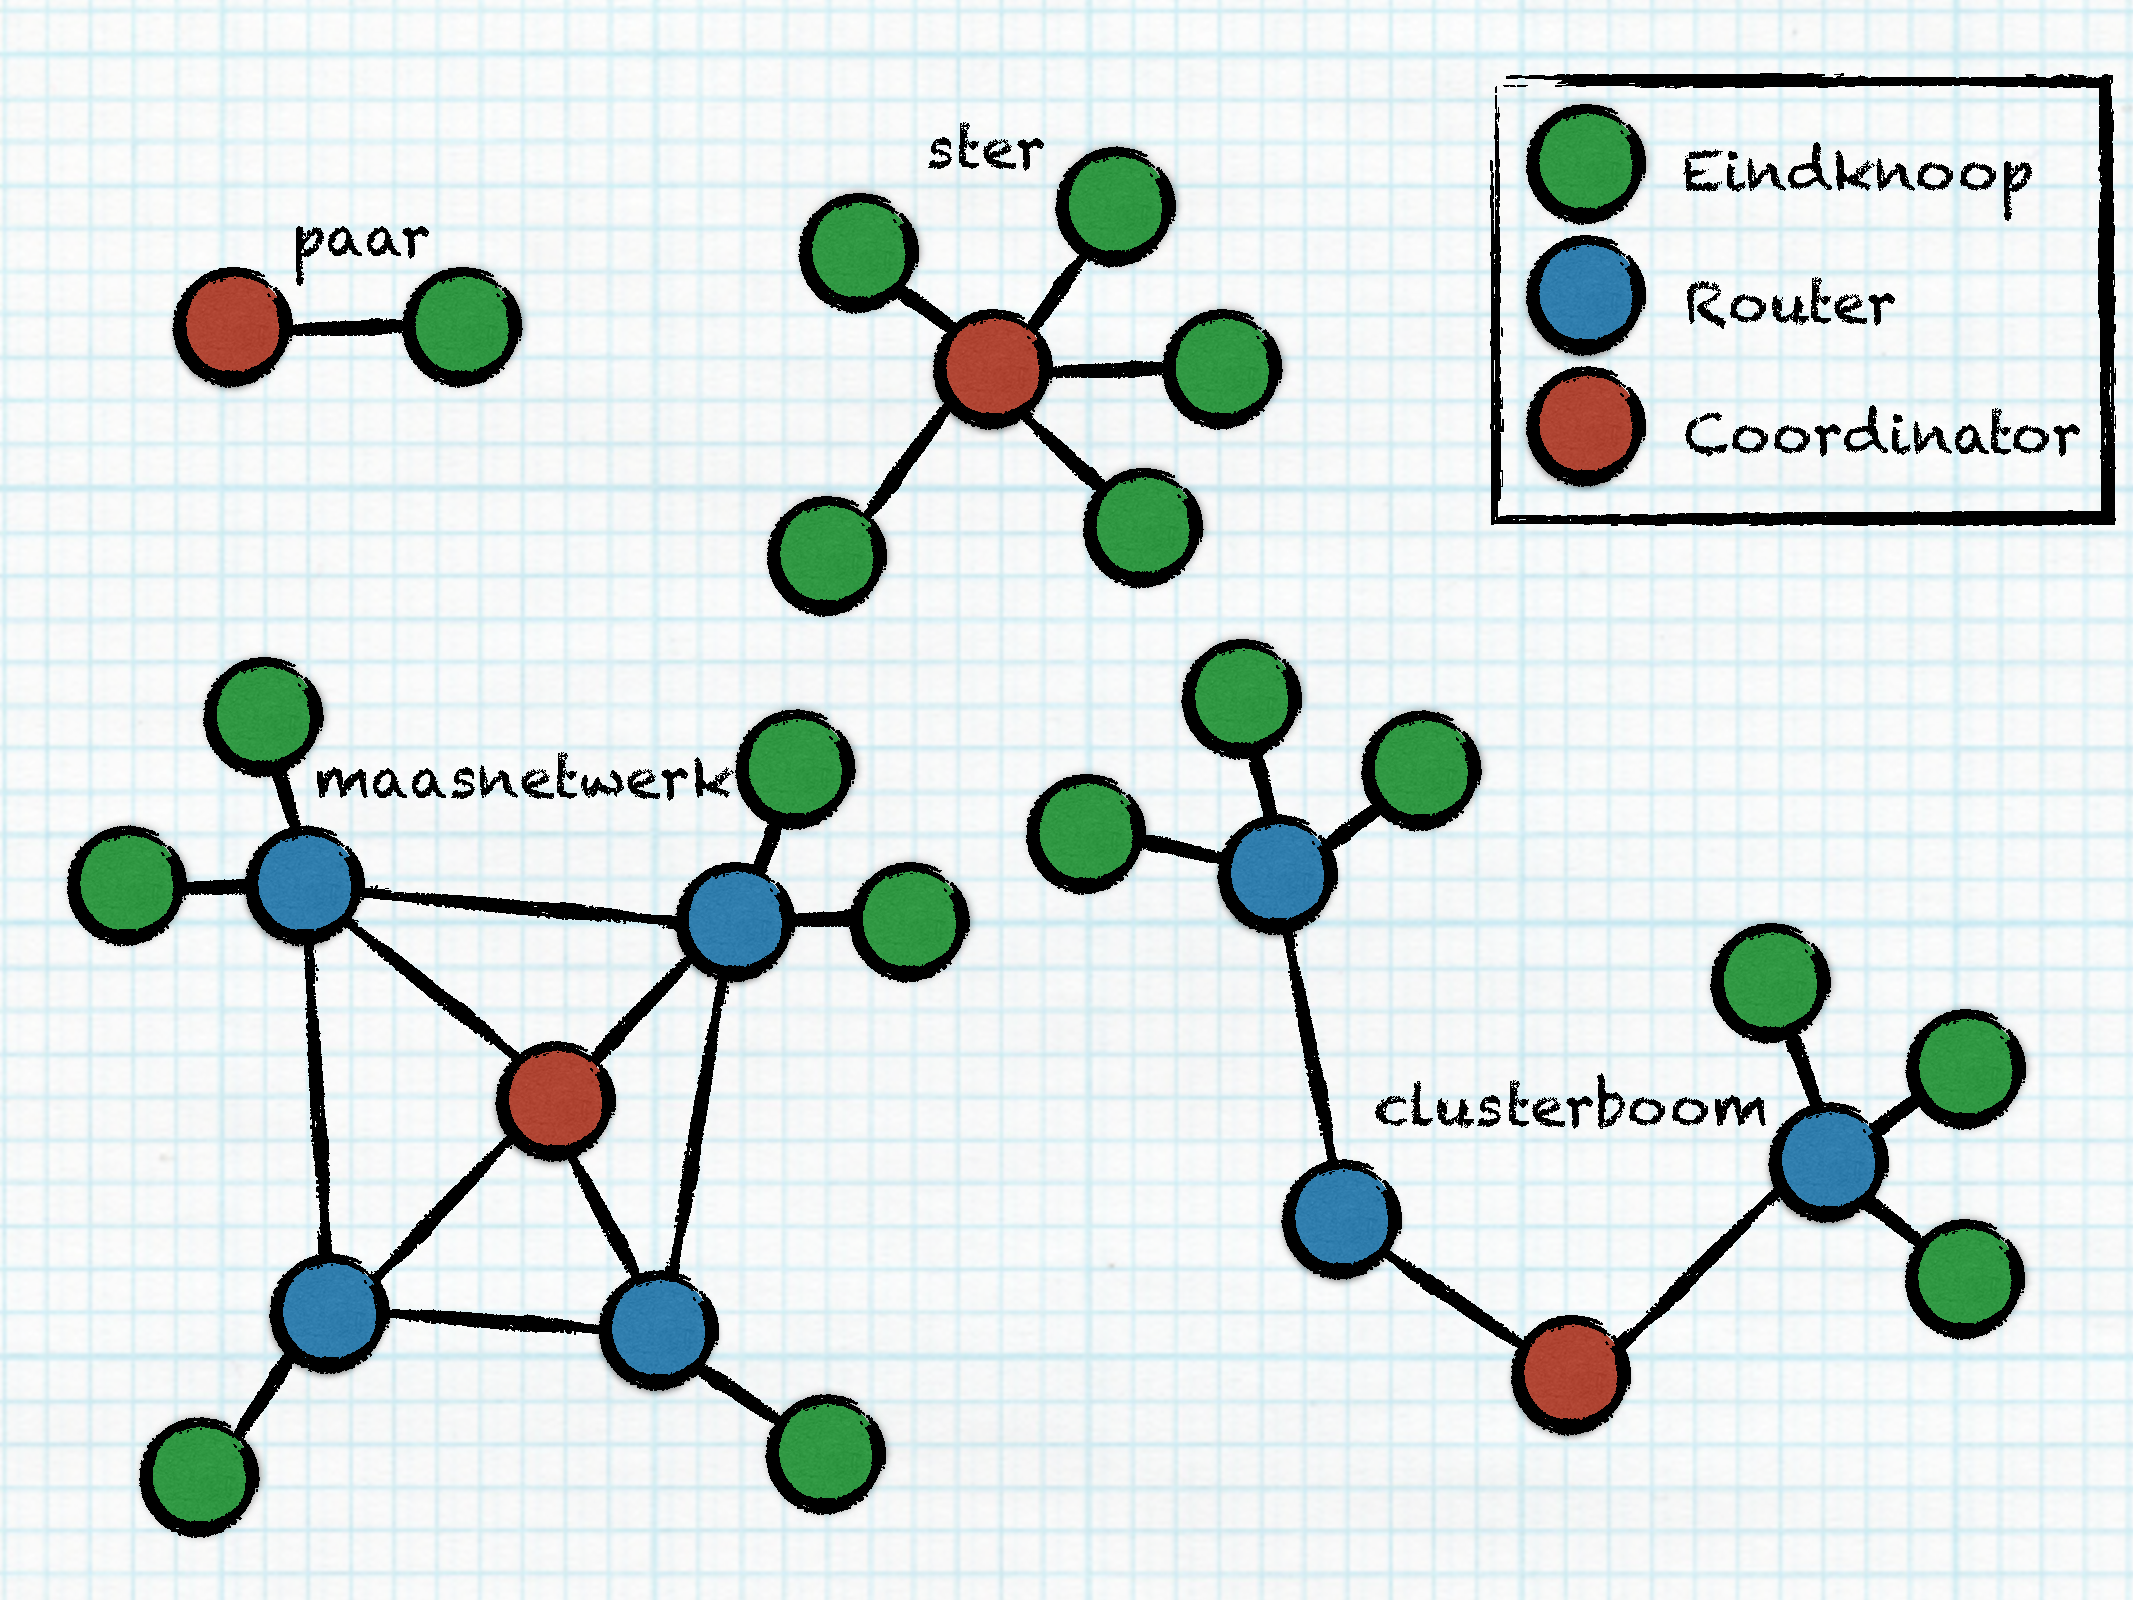
\includegraphics[width=0.7\linewidth]{resources/topology.pdf}
  \caption[Verschillende mogelijke netwerktoplogie\"en]{Verschillende mogelijke
  netwerktoplogie\"en (Bron:\citep{oreilly2010buildingwsn})}
  \label{fig:topologie}
\end{figure}

Het lijkt evident, maar elke knoop, in eender welke topologie, heeft een eigen,
uniek adres, eigenlijk meerdere. Zo heeft een ZigBee-knoop een uniek adres
binnen het netwerk waaraan het deelneemt. Dit adres wordt door de co\"ordinator
van het netwerk toegekend aan een knoop wanneer deze toetreedt tot het netwerk.
Dit \emph{netwerkadres} bestaat uit 16 bits en laat dus toe om 65534 (uit
$2^{16} = 65536$) verschillende adressen toe te kennen. Het adres
\ttt{0x0000}\footnote{We hanteren voor de notatie van adressen de hexadecimale
voorstelling. Elk cijfer stelt een groep van 4 bits voor. 4 groepen stellen zo
een 16 bit adres voor.} reserveert de co\"ordinator voor zichzelf en het adres
\ttt{0xFFFE} wordt typisch gebruikt als het zgn. \emph{broadcast adres}, het
adres waarnaar een bericht gestuurd wordt dat bij alle andere knopen dient
afgeleverd te worden.

Daarnaast heeft elke ZigBee-radio ook een adres dat gegarandeerd overal uniek
is. Dit bestaat uit 64 bits en wordt samengesteld uit twee delen: een eerste
deel beslaat de eerste 32 bits en is voorbehouden voor een unieke identificatie
van de producent. De volgende 32 bits is een uniek nummer binnen de productie
van de producent. Een netwerk zal veelal uit sensoren met dezelfde draadloze
radio's bestaan. Het is daarom logisch dat er gebruik gemaakt wordt van een
\emph{netwerkadres}, dat slechts 16 bits groot is en dus een aanzienlijke
besparing aan geheugen kan opleveren.

Naast de adressen van de knopen is er ook nog het zogenaamde \emph{personal
area network (PAN)} adres. Dit is een unieke identificatie van het netwerk dat
door de co\"ordinator georganiseerd wordt. Ook dit is een 16 bit adres en laat
dus toe om 65536 netwerken op te bouwen.

Tot slot kunnen ZigBee-radio's ook gebruik maken van 12 verschillende
\emph{kanalen}, zodat de volledige adresstructuur bestaat uit een kanaal, een
PAN adres en een netwerkadres.

\section{Beveiligen van sensorknopen}
\label{section:beveiligen}

Het beveiligen van sensorknopen is, in tegenstelling tot de beveiliging van
klassieke computers, bijzonder moeilijk. De computers waar onze emails, foto's
en andere kostbare documenten opgeslagen zijn, zijn uitgerust met een
virusscanner, firewall\dots Dit is mogelijk omdat ze voorzien zijn van een
constante stroomvoorziening, krachtige processor en veel geheugen. Ze zijn
tevens fysiek beschermd door ons huis of het datacenter van onze leverancier
van internetdiensten.

In \citep{dargie2010fundamentals} wordt een goed overzicht gegeven van de
uitdagingen die het beveiligen van DSN met zich meebrengen, in vergelijking met
klassieke netwerken. Een sensorknoop heeft geen constante stroomvoorziening en
moet het veelal stellen met een zeer beperkte batterij. Verder ligt de
sensorknoop meestal letterlijk \emph{ten velde} en is fysiek toegankelijk voor
nagenoeg iedereen.

Er is ook geen centraal punt waar alle communicatie gegarandeerd passeert. Het
enige communicatiemedium is het draadloze netwerk en via die weg kan men steeds
rechtstreeks contact leggen met elke afzonderlijke knoop, zonder dat de
meerderheid van andere knopen dit ooit merkt. Tot slot is het belangrijk voor
ogen te houden dat een draadloos communicatiemedium inherent fouten met zich
meebrengt, en dat berichten verloren kunnen gaan.

\subsection{CIA, AAA en andere beveiligingsprincipes}
\label{subsection:cia}

Beveiliging is een zeer ruim begrip dat veel aspecten overspant. Het is
belangrijk dit voor ogen te houden wanneer we over beveiliging spreken.
Theoretische modellen kunnen hierbij helpen. In deze sectie introduceren we
enkele van deze modellen die kunnen helpen om over beveiliging van DSN te
praten.

Wanneer men spreekt over het beveiligen van computers en netwerken, wordt
dikwijls gerefereerd naar het CIA-beveiligingsmodel. Dit letterwoord staat
voor: vertrouwelijkheid (\emph{confidentiality}), integriteit en
beschikbaarheid (\emph{availability}).

\begin{description}

  \item[Vertrouwelijkheid] Om \emph{vertrouwelijkheid} te garanderen moet
  beveiliging de nodige voorzieningen treffen om er voor te zorgen dat bv. een
  bericht enkel door de bedoelde bestemmeling kan begrepen worden.
  
  \item[Integriteit] Onder \emph{integriteit} verstaat men het principe dat dat
  bericht dan weer niet mag gewijzigd kunnen worden, of dat de bedoelde
  bestemmeling van het bericht ten minste kan valideren dat er aan het bericht
  niets gewijzigd is. 
  
  \item[Beschikbaarheid] Maar beveiliging moet ook de \emph{beschikbaarheid}
  van onderdelen van het netwerk garanderen, om er zeker van te zijn dat dit
  laatste zijn diensten kan blijven aanbieden.

\end{description}

Het CIA-model is zonder meer een belangrijke basis, maar er ontbreken nog veel
belangrijke aspecten. In \citep{rfc:3198} wordt een gestandaardiseerde
terminologie voorgesteld voor het defini\"eren van een beveiligingsbeleid.
Naast de drie hoofdpijlers van het CIA-model vinden we zo ook nog een ander
belangrijk model, namelijk het AAA model voor autorisatie bij
internet-gerelateerde diensten (\emph{triple A}) \citep{rfc:2904}. De afkorting
staat voor authenticatie, autorisatie en vaststellen (\emph{accounting})

\begin{description}

  \item[Authenticatie] Via \emph{authenticatie} kan de identiteit van een
  gebruiker of apparaat vastgesteld worden, zodat eenduidig kan bepaald worden
  van wie bv. een bericht in het netwerk komt.
  
  \item[Autorisatie] \emph{Autorisatie} is daarentegen het proces waarbij
  nagegaan wordt of een gebruiker waarvan de authenticiteit is vastgesteld, een
  bepaalde handeling \emph{mag} uitvoeren.
  
  \item[Vaststellen] Ten slotte biedt het \emph{vaststellen} van alle
  gebeurtenissen en beslissingen binnen het beveiligde domein, een belangrijke
  bron van informatie om een beleid verder te verfijnen en eventueel bij te
  sturen.

\end{description}

In het kader van beveiliging wordt typisch ook gesproken over een \emph{beleid}
(\emph{policy}), waarin de regels zijn opgenomen waaraan alle spelers binnen
het te beveiligen domein zich dienen te houden. Het AAA model hanteert een
beleid als zijn centrale gegeven en definieert componenten zoals een
\emph{policy information point} (PIP), \emph{policy decision point} (PDP) en
een \emph{policy enforcement point} (PEP). Deze componenten kunnen aanduiden
waar de verantwoordelijkheid ligt om respectievelijk de juiste informatie aan
te leveren omtrent het beleid, beslissingen te treffen volgens het beleid en
deze beslissingen effectief uit te voeren.

\begin{description}

  \item[Onweerlegbaarheid] Naast deze aspecten, is er ook nog het principe van
  onweerlegbaarheid (\emph{non-repudiation}). Door garanties omtrent
  \emph{onweerlegbaarheid} in te bouwen, kan een ontvanger er zeker van zijn
  dat een zender van een bericht dit bericht effectief verstuurd heeft.

\end{description}

Een aantal gekende technieken bieden klassiek oplossingen voor verschillende
van de hoger vermelde principes: Digitale handtekeningen kunnen helpen bij het
garanderen van de \emph{authenticiteit}, \emph{onweerlegbaarheid} en
\emph{integriteit} van een boodschap. Cryptografie kan logischerwijs de
\emph{vertrouwelijkheid} van berichten garanderen, maar kan ook aan de hand van
publieke en private sleutels de \emph{authenticiteit} vaststellen. Berichten
kunnen alleen met de andere sleutel van het paar versleuteld worden.

In hoofdstukken \ref{chapter:achtergrond} en \ref{chapter:probleemstelling}
gaan we dieper in op de typische eigenschappen van sensorknopen en belichten we
tal van beveiligingsrisico's waaraan DSN blootgesteld zijn. Aan de hand van de
zonet beschreven principes zullen we zien dat DSN inherent moeilijk te
beveiligen zijn en dat het nagenoeg onmogelijk is om inbraken te vermijden.

\subsection{Inbraakdetectie}
\label{subsection:detection}

Indien het vermijden van inbraken nagenoeg onmogelijk is, moet een belangrijke
tweede beveiligingslinie opgetrokken worden: inbraakdetectie.

Indien we niet weten dat een inbraak heeft plaatsgevonden, zullen we enkel een
vals gevoel van veiligheid hebben. Het is niet omdat we het niet weten, dat ze
er niet zijn. Misschien moeten we zelfs durven stellen dat het belangrijker is
om meer te weten dan te vermijden.

Inbraakdetectie is typisch de stille vennoot in een beveiligingsverhaal. Daar
waar bv. een firewall of authenticatieserver actieve toegang ontzegt, zal een
inbraakdetectiesysteem (IDS) typisch geen actieve rol spelen. Het IDS zal
eerder bewijsmateriaal verzamelen om een inbraakpoging te documenteren. Uit
deze informatie kunnen dan bijsturingen aan het beleid aangebracht worden,
waardoor actieve componenten in de toekomst wel in staat zijn om gelijkaardige
inbraakpogingen te verijdelen.

Deze architectuur legt al snel een belangrijk pijnpunt bloot: in een klassiek
netwerk wordt het netwerk beschermd aan de rand. De firewall schermt het
interne netwerk af van aanvallen van buiten. Als een spreekwoordelijke muur van
vuur wordt elke toegang tot het netwerk gelouterd en ongewenste berichten
worden onherroepelijk \emph{verbrand} v\'o\'or ze het netwerk kunnen betreden.

Het IDS wordt daarom typisch ook op het interne netwerk aangesloten daar waar
alle netwerkverkeer dat door de firewall wordt doorgelaten, passeert. Aanvallen
die toch nog door de firewall geraken, kunnen nog door het IDS gedetecteerd
worden.

Dit lijkt op het eerste zicht een tegenspraak. Indien het IDS deze aanvallen
kan detecteren, waarom wordt deze kennis dan niet gebruikt op het niveau van de
firewall? De reden ligt in de natuur van de firewall. Deze werkt immers
hoofdzakelijk op netwerkniveau en bekijkt elk netwerkpakket op zich. Aanvallen
zijn soms een samengang van verschillende pakketten, die typisch op zich zelfs
perfect legaal zijn. Het draait hier hoofdzakelijk om de inhoud van de
pakketten en de analyse vraagt dikwijls een kennis van de toepassingen waarmee
gecommuniceerd wordt. Soms kan slechts aan de inhoud van antwoorden uit het
interne netwerk opgemaakt worden dat er een inbraak plaatsgevonden heeft. Deze
complexiteit is te groot om op het niveau van een firewall te realiseren.

De resultaten van een IDS zullen dikwijls eerder leiden tot verbeteringen aan
de toepassingen binnen het interne netwerk, zodat deze niet meer vatbaar zijn
voor het soort inbraken dat gedetecteerd werd.

Wanneer we dit nu afspiegelen op een DSN, merken we dat enkele fundamentele
principes zo'n architectuur onmogelijk maken: een DSN heeft geen afgebakende
netwerkrand, er is geen uniek punt waar alle netwerkverkeer passeert en waar
een firewall zou kunnen ge\"introduceerd worden, laat staan dat er een manier
zou zijn om al het interne verkeer op \'e\'en enkele plaats te analyseren.

Binnen een DSN is het letterlijk elke knoop voor zichzelf: elke knoop kan
immers van buitenaf benaderd worden zonder dat een aanvaller moet passeren
langs een centraal controlepunt.

\section{Probleemstelling}
\label{section:probleem}

DSN en sensorknopen op zich zijn geen makkelijke klanten wat beveiliging
betreft. Enerzijds hebben ze onvoldoende middellen om zich te beschermen en
anderzijds is hun situatie zo dat het letterlijk elke knoop voor zichzelf is en
dat ze nauwelijks kunnen vertrouwen op hun collega's.

In dit kader moeten gebruikers van een DSN eisen dat er voldoende garanties
worden gegeven zodat ze zich voldoende verzekerd voelen om intieme informatie
toe te vertrouwen aan deze netwerken.

Aangezien het haast onmogelijk is om inbraakpogingen te verijdelen is het van
groot belang dat men in staat is om ze ten minste vast te stellen. Het
introduceren van een IDS in het DSN is echter een directe aanval op de
essenti\"ele functionaliteit van een sensorknoop, waardoor de mogelijkheden
sterk beperkt worden.

\section{Doelstelling}
\label{section:doelstelling}

Zoals we zullen zien in sectie \ref{section:related}, ligt in de literatuur
betreffende ``inbraakdetectie in draadloze sensornetwerken'' de nadruk in
hoofdzaak op het detecteren van specifieke aanvallen of het vaststellen van
anomalie\"en in het verwachte gedrag van sensorknopen en/of het netwerk dat hen
verbindt.

Deze werken stellen tevens dat het een nagenoeg onmogelijke taak is om alle
benodigde detectiemechanismen effectief te implementeren. Dit is logisch,
gegeven het beperkte aanbod aan middelen die sensorknopen typisch ter
beschikking hebben. Zo zou bv. een exhaustieve lijst van aanvalspatronen
slechts in sensorknopen met een groot geheugen kunnen opgeslagen worden en
zouden de berekeningen die nodig zijn om bepaalde anomalie\"en te detecteren
gewoonweg te veel energie verbruiken.

Als in dit stadium van onderzoek naar systemen om inbraken te detecteren het
niet mogelijk is om een sluitend IDS voor een DSN te ambi\"eren, lijkt het
opportuun om een stap terug te zetten en de focus te leggen op de middelen die
nodig zijn om de reeds beschreven, en mogelijk ook toekomstige algoritmen, te
realiseren. Is het mogelijk om een kader te cre\"eren dat een ontwikkelaar van
een sensorknoop in staat stelt om een selectie van de in de literatuur
beschreven oplossingen te implementeren? Kan hij een IDS toevoegen aan zijn DSN
zonder een diepgaande analyse van de onderzoeksliteratuur en zonder zich zorgen
te moeten maken over de onderliggende interactie met andere knopen, het
vergaren en opvragen van informatie op systeem-niveau\dots?

Deze masterproef wil zo'n kader ontwerpen, een prototype implementeren en de
impact bepalen. Daartoe bekijken we eerst enkele typische voorbeelden van
inbraakdetectiealgoritmen, waaruit de functionele en technische vereisten
gedistilleerd worden. Vervolgens stellen we een architectuur voor die aan deze
vereisten kan voldoen. Aan de hand van een prototype gaan we tot slot na wat de
impact is met betrekking tot geheugen en rekenkracht.

De voordelen van een raamwerk zijn legio: een herbruikbaar raamwerk neemt
zorgen, gemeenschappelijk aan de verschillende oplossingen, weg en kan zorgen
voor een betere implementatie. Door middel van een goedgekozen technische
architectuur kan tevens platformonafhankelijheid nagestreefd worden.

%!TEX root=masterproef.tex

\chapter{Achtergrond}
\label{chapter:achtergrond}

In het inleidende hoofdstuk werd het concept WSN al kort ge\"introduceerd. In
dit hoofdstuk wordt het kader geschetst waarbinnen we op zoek gaan naar
antwoorden.

Sectie \ref{section:landscape} brengt het landschap van draadloze
sensornetwerken in kaart: wat typeert en onderscheidt hen van andere netwerken?
Wie is de aanvaller en wat zijn zijn doelen? Waarom is het vaststellen van
inbraken een belangrijk onderzoeksdomein?

Sectie \ref{section:related} gaat in op gerelateerd onderzoek. Een doelstelling
van deze masterproef is ook het in kaart brengen van de mogelijkheden en
beperkingen betreffende al beschreven methodes om inbraken vast te stellen.

Bij de beschrijving van de verschillende oplossingen zal tevens kritisch
nagegaan worden in hoeverre deze in een realistische situatie effectief
bijdragen tot het detecteren van inbreuken in het netwerk.

%!TEX root=masterproef.tex
\section{Draadloze sensornetwerken}
\label{section:landscape}

\TODO

Zeer terecht stelt \cite{perrig2004security} dat de eerste zorg omtrent de
beveiliging van draadloze sensor netwerken een veilige manier om de groep van
sensoren te beheren is. De manier waarop nieuwe knopen in het netwerk worden
opgenomen en de beveiliging van de onderlinge communicatie is van primordiaal
belang. Voorkomen is beter dan genezen.

Maar we moeten ook realistisch zijn. Geen door mensenhanden gemaakt systeem is
feilloos en nagenoeg elk ge\"informatiseerd system zal met de nodige inzet en
moeite veroverd kunnen worden. Op dat ogenblik is het belangrijk dat er een
tweede verdedigingslinie is: de inbraak detectie.

\TODO

In \cite{zhang2000intrusion} wordt een zeer algemene, maar zeer correcte
definitie gegeven van inbraak detectie.

\begin{quote}
Intrusion detection therefore involves capturing audit data and reasoning
about the evidence in the data to determine whether the system is under attack.
\end{quote}

%!TEX root=masterproef.tex
\section{Gerelateerd onderzoek}
\label{section:related}

Het detecteren van inbraken komt dikwijls neer op het detecteren van abnormaal
gedrag of anomalie\"en. Er zijn verschillende manieren hoe normaal gedrag kan
gedefinieerd worden elk met hun voor- en nadelen, beperkingen en successen.
(\ref{subsection:anomaly}).

Met de komst van draadloze sensornetwerken moesten veel klassieke
beveiligingstechnieken herbekeken worden. De schaal waarop deze netwerken
opereren, maar vooral de fysieke toegankelijkheid, waren parameters die niet
als problemen ervaren werden in meer klassieke computernetwerken. Hierdoor
moesten fundamentele eigenschappen die niet langer eenvoudig technologisch
afgedekt konden worden, opnieuw gedefinieerd worden. Zo leiden de hoge graad
van distributie en de beperkte mogelijkheden tot onderlinge communicatie al
snel tot de concepten reputatie en vertrouwen (\ref{subsection:reputation}).

Anderzijds zal blijken dat een knoop op zich niet eenvoudig kan beslissen of
hij al dan niet een andere knoop vertrouwt. Knopen zullen - en dit is eigenlijk
een fundamentele eigenschap van draadloze sensornetwerken - moeten samenwerken.
De nood voor co\"operatieve algoritmen (\ref{subsection:cooperation}) is een
belangrijke volgende bouwsteen.

Hoe voeden we dit co\"operatief opgebouwd vertrouwen in een omgeving waar een
aanvaller fysieke toegang heeft tot elke knoop en zowel de vluchtige als de
programmageheugens kan benaderen en wijzigen? Een logische piste is om op zoek
te gaan naar een manier om de programmacode die op een knoop ge\"installeerd is
te valideren voordat deze aangeroepen wordt. Is het eigenlijk wel mogelijk om
aan software-attestatie (\ref{subsection:attestation}) te doen? Eigenlijk is
software-attestatie slechts een specifieke vorm van het nagaan van de
integriteit van een bepaald aspect van een knoop. In dit geval gaat het om de
inhoud van het geheugen. In het algemeen kan dit beschouwd worden als het
opsporen van anomalie\"en.

Naast detectiealgoritmen, zijn ook pogingen gedaan om allesomvattende
raamwerken te cre\"eren. Deze zouden het detecteren en verijdelen van aanvallen
makkelijker moeten maken. (\ref{subsection:frameworks}).

Enkele werken die een goed overzicht bieden van de stand van zaken met
betrekking tot inbraakdetectie in WSN zijn o.a. \citep{mishra2004intrusion} en
\citep{alrajeh2013intrusion}. Naast grote overlappingen met de hierna
gepresenteerde topics, bevatten ze nog andere voorbeelden en/of indelingen
omtrent deze materie.

%!TEX root=masterproef.tex

\subsection{Detecteren van anomalie\"en}
\label{subsection:anomaly}

Een anomalie is een afwijking van een normaal verloop van gebeurtenissen of
iets of iemands gedrag. Een knoop uit een DSN heeft een redelijk eenvoudig en
constante levensloop. Typisch zal een knoop op regelmatige tijdstippen
\emph{wakker worden}, waarden opmeten aan de hand van zijn sensoren en deze
waarden doorsturen naar een centrale locatie. Verder zal een knoop, als
onderdeel van het netwerk, tevens zulke waarden van andere knopen doorsturen.
Dit patroonmatige gedrag kan ge\"identificeerd worden en in een model verwerkt
worden. Op basis van zulk een model kan vervolgens nagegaan worden of de acties
van een knoop op een gegeven moment in lijn zijn met het model of dat er sprake
is van een anomalie.

Zulk een afwijking van het verwachte gedrag kan wijzen op veranderingen van
buitenaf. Deze kunnen op hun beurt veroorzaakt zijn door een aanval op het
netwerk. Aangezien we niet alle communicatie van en naar knopen kunnen
onderscheppen en eventuele aanvallen kunnen detecteren, kunnen
anomaliegebaseerde dectectiemechanismen helpen om op basis van neveneffecten
toch aanvallen te detecteren, of althans toch de gevolgen ervan.

\subsubsection*{Anomali\"en, afwijkingen, aberraties}
\label{subsubsection:outlier}

\citep{zhang2010outlier} is een excellent overzicht van methoden om anomali\"en,
afwijkingen of aberraties (\emph{outliers}) te detecteren in een reeks
van metingen. Het belicht enerzijds de fundamentele technieken die ter
beschikking staan om deze aberraties op te merken maar tracht ook een
classificatie en taxonomie op te stellen hiervoor.

De auteurs stellen dat het detecteren van afwijkingen behoort tot het domein
van \emph{datamining} en dat het in die context reeds uitvoerig onderzocht is,
evenals binnen disciplines as statistiek, machinaal leren, informatie
theorie \dots. Aangezien het kunnen uitsluiten van afwijkingen de verwerking
van de overblijvende meetresultaten sterk positief be\"invloed is het in het
kader van DSN uitermate interessant.

Toch kan eerder onderzoek opnieuw niet eenvoudig toegepast worden in het kader
van DSN. De beperkte middelen van de sensorknoop schrappen al veel van de
klassieke oplossingen die bv. gecentraliseerd werken. De overdaad aan
communicatie die nodig is om voldoende gegevens te centraliseren voor
verwerking is niet realistisch in het kader van een DSN. Ook zijn veel van de
algoritmen typisch niet ontwikkeld met de beperkte rekenmogelijkheden van
sensorknopen. De conclusie is dat er een balans moet gevonden worden tussen de
mogelijkheden van datamining algoritmen voor het detecteren van afwijkingen en
de verhouding van hun noden ten opzichte van de middelen van de knopen.

\subsubsection*{Neurale netwerken}
\label{subsubsection:neuralnetworks}

Wanneer men denkt aan het vastleggen van een patroon en het controleren of een
bepaalde situatie voldoet aan dat patroon wordt in informatiecakringen ook snel
verwezen naar neurale netwerken. Neurale netwerken kunnen immers
\emph{getraind} worden door middel van een aantal goede (en slechte)
voorbeelden, waarna nieuwe voorbeelden kunnen gecatalogeerd worden als ook goed
of slecht. De complexiteit van het bepalen van deze beslissing is typisch
redelijk eenvoudig en lijkt zich daarom uitermate goed te lenen voor het
detecteren van anomalie\"en door sensorknopen.

In \citep{ramesh2012wireless} volgen de auteurs deze denkpiste, maar stellen
tevens dat er betere methoden bestaan. Ze trachten twee specifieke aanvallen
het hoofd te bieden: DoS en passieve informatie vergaring en vergelijken
hierbij een aanpak op basis van een neuraal netwerk en hun eigen aanpak op
basis van encryptie op basis van symmetrische sleutels.

Ofschoon dat sommige van hun veronderstelling na\"ief zijn (zo baseren ze zich
op een gedeelde geheime sleutel van 8 bits), toont hun werk wel aan dat een
aanpak met neurale netwerken eenvoudig te realiseren is en een valabele piste
kan zijn om anomaliedetectie te doen.

\subsubsection*{Voorspellingen}
\label{subsubsection:predictions}

Waar neurale netwerken in staat zijn om op basis van voorbeelden een nieuwe
situatie te catalogeren, kan men aan de hand van een Markov model
voorspellingen doen over de toekomst.

Het is deze piste dat onderzocht wordt in \citep{zhijie2012intrusion}. Opnieuw
betreft het een poging om DoS aanvallen te detecteren. De bedoeling is dat
sensorknopen individueel bepalen of er een DoS aanval bezig is. Volgens de
auteurs is dit mogelijk aan de hand van een Markov model dat het netwerkverkeer
voorspelt.

Het model wordt zo geconstrueerd dat er een verband ontstaat tussen de toestand
van een knoop in relatie tot het tijdstip en de verwachtte hoeveelheid gegevens
die verstuurd zouden kunnen worden.

Het idee achter het artikel lijkt een mogelijke piste, maar omtrent veel
belangrijke details blijven echter zeer vaag, waardoor de volledige toedracht
van het algoritme niet eenduidig ingeschat kan worden. Zo wordt bv. nauwelijks
ingegaan op wat de toestand van een knoop juist bepaalt of hoe de
hoeveelheid gegevens die verstuurd kunnen worden wanneer een knoop zich in een
bepaalde toestand bevindt, bepaald wordt.

%!TEX root=masterproef.tex

\subsection{Reputatie en vertrouwen}
\label{subsection:reputation}

De probleemstelling dat knopen in het netwerk elkaar niet langer kunnen
vertrouwen, zette verschillende onderzoekers aan tot het zoeken naar
oplossingen gebaseerd op reputatie en vertrouwen.

\citep{ganeriwal2008reputation} beschrijft een architectuur gebaseerd op
observaties door knopen van de acties van andere knopen in het kader van acties
van zichzelf of derde knopen. Figuur \ref{fig:reputation-cooperation} toont de
situaties die beschouwd worden: in \ref{fig:reputation-cooperative-node} zal
een co\"operatieve knoop (C) alle boodschappen die via hem verzonden worden
door een zendende knoop (Z) effectief doorsturen naar een verdergelegen
ontvangende knoop (O). De verzender van de boodschap, alsook andere naburige
knopen (B) kunnen deze actie vaststellen. In
\ref{fig:reputation-uncooperative-node} daarentegen zal een een
niet-co\"operatieve knoop (NC) deze boodschappen niet verder versturen of zelfs
aanpassen.

\begin{figure}
\centering
\begin{subfigure}{.49\textwidth}
\centering
  \includegraphics[width=.8\linewidth]{./resources/cooperative.pdf}
  \caption{Co\"operatieve knoop}
  \label{fig:reputation-cooperative-node}
\end{subfigure}
\begin{subfigure}{.49\textwidth}
\centering
  \includegraphics[width=.8\linewidth]{./resources/non-cooperative.pdf}
  \caption{Niet-co\"operatieve knoop}
  \label{fig:reputation-uncooperative-node}
\end{subfigure}
\caption{Beschouwde situaties bij al dan niet co\"operatieve knopen}
\label{fig:reputation-cooperation}
\end{figure}

Op basis van deze situatie stellen de auteurs dat de reputatie van een knoop
kan weergegeven worden aan de hand van een beta distributie. Bijlage
\ref{appendix:reputation} bespreekt de mathematische onderbouw hiervan.

De auteurs vermelden zelf een zeer belangrijk probleem: omdat knopen constant
moeten luisteren naar de acties van naburige knopen, moeten zij constant actief
zijn. Dit is een zeer nadelig uitgangspunt voor systemen die typisch trachten
zuinig om te springen met hun energie.

Maar de architectuur heeft ook inherente problemen en laat kwaadwillige
partijen toe om - mits kennis van de parameters - net onder de radar te
opereren. We illustreren dit met de simulatie zoals deze uitgevoerd werd door
de auteurs.

De evolutie van een volledige co\"operatieve of volledige niet-co\"operatieve
knoop wordt weergegeven in figuur \ref{fig:reputation-paper}. Een eigenschap
van het algoritme is dat pas na een tiental (louter positieve) observaties een
knoop de drempelwaarde van vertrouwen overschrijdt.

\begin{figure}[ht]
\centering
\begin{subfigure}{.49\textwidth}
  \centering
  \includegraphics[width=.9\linewidth]{./resources/reputation-paper.pdf}
  \caption{Co\"operatieve en niet-co\"operatieve knopen}
  \label{fig:reputation-paper}
\end{subfigure}
\begin{subfigure}{.49\textwidth}
  \centering
  \includegraphics[width=.9\linewidth]{./resources/reputation-with-failure.pdf}
  \caption{Falende knopen (100 simulaties)}
  \label{fig:reputation-with-failure}
\end{subfigure}
\caption{Impact van falende knopen op evolutie van vertrouwen}
\label{fig:reputation-paper-with-failure}
\end{figure}

Deze eigenschap kan echter misbruikt worden zoals aangetoond wordt in figuur
\ref{fig:reputation-with-failure}. Stel dat een knoop $j$ te kampen heeft met
falende hardware, waardoor 5\% van zijn transmissies verloren gaan en daarom
ook niet opgemerkt kunnen worden door andere knopen.

We merken op dat deze knoop, zelfs met 5\% niet-co\"operatieve observaties, na
een twintigtal observaties toch boven de drempelwaarde uitkomt en door de
beschouwende knoop aanvaard wordt als betrouwbaar.

Vanuit een operationeel standpunt gezien is dit in eerste instantie een
positief effect. Indien een knoop \emph{slechts} 5\% faalt zal deze toch als
co\"operatief beschouwd worden en de goede werking van het netwerk niet
fundamenteel in het gedrang brengen - vanuit een inbraakdetectie-oogpunt gezien.

Maar stel dat deze 5\% niet-co\"operatieve acties geen falen zijn en dat de
doorgestuurde boodschappen niet verloren gaan, maar met opzet lichtjes
gewijzigd worden. 5\% kan een significante vertekening van metingen van een
netwerk betekenen en zo de werking van het hele netwerk ondermijnen.

Figuur \ref{fig:reputation-malicious} gaat slechts een kleine stap verder en
toont het effect van falende (of malafide) knopen die pas falingen vertonen
nadat ze het vertrouwen hebben gekregen van een knoop. We merken op dat nu zelfs
10\% falingen zeer lang het vertrouwen kunnen behouden.

\begin{figure}[ht]
 \centering
 \includegraphics[width=.5\linewidth]{./resources/reputation-malicious.pdf}
 \caption{Falende knopen met vertraging van 15 pakketten (100 simulaties)}
 \label{fig:reputation-malicious}
\end{figure}

Dit elementaire voorbeeld toont duidelijk aan dat het vaststellen van een
reputatie op basis van externe observaties een zeer delicaat onderwerp is dat
zeer gevoelig is voor manipulatie op basis van kennis van de interne
parameters. Dit laatste is dan weer net \'e\'en van d\'e problemen waar
draadloze sensornetwerken mee kampen omdat knopen vrij eenvoudig kunnen
weggenomen, ge\"inspecteerd, gewijzigd en teruggeplaatst worden.

%!TEX root=masterproef.tex
\subsection{Co\"operatieve algoritmen}
\label{subsection:cooperation}

Het detecteren van abnormaal gedrag, dat op zijn beurt een indicatie kan zijn
van een (poging tot) inbraak door \'e\'en knoop is \'e\'en ding, als netwerk
van knopen tot een consensus komen en met meer zekerheid een verdachte knoop
uitsluiten is een heel ander ding.

Een veel voorkomend onderwerp is dat van co\"operatie tussen knopen, waarbij in
overleg bepaald wordt of en welke andere knoop uitgesloten moet worden uit het
netwerk. In \citep{krontiris2009cooperative} wordt hiertoe eerst langs een
theoretische weg gezocht naar de nodige en voldoende voorwaarden voor
inbraakdetectie. Vervolgens wordt er een praktisch omkaderend algoritme
voorgesteld om op co\"operatieve manier aan inbraakdetectie te doen.

Zowel dit theoretische model als het praktische algoritme vormen een
interessante bron van informatie. Het theoretische model kan helpen bij het
analyseren van andere co\"operatieve oplossingen en het praktische algoritme
biedt een algemeen raamwerk voor het implementeren van co\"operatieve
strategie\"en.

Bijlage \ref{appendix:idp-cooperation} gaat in meer detail in op de
mathematische onderbouw van het zgn. \emph{Intrusion Detection Problem} (IDP).
Naast een theoretisch model wordt tevens een algoritme voorgesteld dat het
mogelijk maakt om op gedistribueerde manier samen te werken en tot een
beslissing te komen aangaande de aanwezigheid van een malafide knoop in het
netwerk.

Het algoritme is een betrekkelijk eenvoudig raamwerk voor een co\"operatieve
aanpak, waarbij knopen zelfstandig beslissen welke andere knopen ze verdenken
en vervolgens gezamenlijk, op een gedistribueerde manier, trachten tot een
consensus te komen welke van de verdachte knopen effectief de aanvaller is.

De kracht van dit raamwerk en het succes ervan hangt natuurlijk sterk af van de
lokale detectiemogelijkheden van de knopen en de accuraatheid hiervan.

\subsubsection*{Risico's}

Het voorbeeld in figuur \ref{fig:idp-examples-2} beslaat een zeer beperkte
scope en de voorwaarden van het IDP kunnen in praktijk niet geverifieerd
worden. We moeten voorzichtig zijn niet te snel conclusies te trekken die in
een ruimere situatie misschien een verkeerd beeld zouden kunnen opleveren.
Figuur \ref{fig:sinkhole-ripple} toont essentieel hetzelfde voorbeeld als dat
van \ref{fig:idp-examples-2}, maar nu met meer knopen rondom het initi\"ele
voorbeeld.

Het routeringalgoritme is gebaseerd op de totale kost van het pad naar het
basisstation en komt daarmee overeen met het MultiHopLQI routering algoritme
beschreven in o.a. \citep{krontiris2008launching}. In dit werk wordt ook de
zgn. \emph{Sinkhole Attack} voorgesteld. We nemen deze aanval als voorbeeld.

\begin{figure}[ht]
\centering
\begin{subfigure}{.49\textwidth}
  \centering
  \includegraphics[width=.8\linewidth]{./resources/sinkhole-before.pdf}
  \caption{Initi\"ele topologie, routes en kosten}
  \label{fig:sinkhole-ripple-1}
\end{subfigure}
\begin{subfigure}{.49\textwidth}
  \centering
  \includegraphics[width=.8\linewidth]{./resources/sinkhole-after.pdf}
  \caption{Knoop $d$ kondigt ``betere'' route aan}
  \label{fig:sinkhole-ripple-2}
\end{subfigure}
\caption{Voorbeeld van het theoretische risico dat kan leiden tot een verkeerde
identificatie van de echte aanvaller}
\label{fig:sinkhole-ripple}
\end{figure}

Stel dat knoop $d$ een \emph{Sinkhole Attack} uitvoert door een zeer lage kost
te adverteren. Hierdoor zal knoop $a$ geneigd zijn om zijn route aan te passen.
Hierdoor zal deze op zijn beurt een veel voordeligere route adverteren en
zullen ook knopen $b$ en $c$ hun route wijzigen en hun gegevens via knoop $a$
versturen.

Ten gevolge van deze route-updates is het mogelijk dat een lokale detector voor
de \emph{Sinkhole Attack} op knopen $a$ en $b$ in werking zal treden. Hierbij
kunnen de knopen alleen hun volledige buurt beschuldigen, omdat het niet
mogelijk is om te detecteren wie de valse boodschappen effectief verstuurd
heeft. Indien de aanvallende knoop $d$ nu ook selectief zijn naburige knoop $a$
beschuldigt, komen we tot dezelfde situatie als in figuur
\ref{fig:idp-examples-2}, echter nu met mogelijk een verkeerd
ge\"identificeerde aanvaller, omdat in deze situatie niet voldaan is aan de
voorwaarden van het IDP.

Dit voorbeeld is, net zoals de vele andere beschreven voorbeelden, uitermate
specifiek en dient louter ter illustratie van het fragiele karakter van een
co\"operatief algoritme. Desalniettemin bieden de concepten en het omkaderende
algoritme ge\"introduceerd in \citep{krontiris2009cooperative} een goed
uitgangspunt voor het beschrijven en implementeren van
inbraakdetectiemechanismen.

\subsubsection*{Groeperen}
\label{subsubsection:grouping}

Een andere aanpak van co\"operatieve algoritmen vertrekt van het groeperen van
knopen. Deze aanpak wordt toegepast door \citep{li2008group}. Groepering
gebeurt op basis van nabijheid en tracht sensoren te groeperen die door hun
locatie gelijkaardige meetwaarden zouden moeten opmeten. De auteurs stellen een
algoritme voor op basis van verschillen, een zgn. delta-algoritme.

Metingen van knopen kunnen nu binnen de groep met elkaar vergeleken worden, en
afwijkende resultaten (zie ook sectie \ref{subsection:anomaly}) kunnen op
statistische wijze beschouwd worden als abnormaal gedrag en op die manier
gerapporteerd worden.

%!TEX root=masterproef.tex
\subsection{Attesteren van software}
\label{subsection:attestation}

Het voorbeeld uit sectie \ref{section:node-capture} toonde al aan dat zelfs het
vluchtige geheugen van een knoop niet veilig is. Als een aanvaller in staat is
om ongemerkt de programma-code van een knoop te bekomen, alsook alle gegevens
die alleen tijdens uitvoering in het geheugen, dan kan deze aanvaller deze code
aanpassen zodat de werking ogenschijnlijk ongewijzigd is, maar dat hij toch
controle heeft over de werking en zo het hele netwerk kan be\"invloeden.

Een zeer logische onderzoeksvraag dient zich al snel aan: ``\emph{Is het
mogelijk om wijzigingen aan het programma van een knoop in het netwerk vast te
stellen?}''. Deze vraag wordt onderzocht binnen het domein van software
attestatie.

\subsubsection*{Werking}

Alle bestaande vormen van software attestatie maken gebruik van een protocol
gebaseerd op het challenge response principe. Als men de integriteit van een
knoop wil vast stellen, zal men aan deze knoop een verzoek sturen om een unieke
samenvatting te maken van zijn inhoud door middel van een cryptografische
hashfunctie, een \emph{checksum}.

De vaststeller beschikt zelf over een versie van de inhoud van de knoop en kan
dezelfde unieke samenvatting berekenen. Door in het initi\"ele verzoek een
\'e\'enmalig te gebruiken code mee te geven, een zgn. \emph{nonce}, en deze
deel te laten uitmaken van de inhoud, kunnen verschillende verzoeken telkens
met een ander, unieke samenvatting beantwoord worden en wordt kan deze
samenvatting niet op voorhand gekend en berekend worden. Figuur
\ref{fig:attestation-process} geeft een overzicht van de werking van software
attestatie en illustreert hoe een wijziging door een aanvaller zich propageert.

\begin{figure}
  \centering
  \includegraphics[width=0.9\linewidth]{resources/attestation-process.pdf}
  \caption{De werking van software attestatie: een aanvaller heeft een
  wijziging kunnen aanbrengen in de programma code op een knoop. Deze wijziging
  propageert zich in de \emph{checksum} en wordt door de vaststeller opgemerkt.}
  \label{fig:attestation-process}
\end{figure}

De inhoud waarvan een samenvatting gemaakt wordt is typisch de programma code
die op de knoop ge\"installeerd werd. Indien een aanvaller deze code kon
wijzigen, zou de samenvatting niet langer overeenkomen met die opgesteld door
de vaststeller en kan deze laatste besluiten om deze gewijzigde code niet te
vertrouwen en de knoop uit te sluiten.

\subsubsection*{Implementaties}

SWATT werd voorgesteld in \cite{seshadri2004swatt}. Het is een attestatie
procedure die een \emph{checksum} berekent over nagenoeg alle geheugenlocaties,
echter wel in willekeurige volgorde. Anderzijds houdt SWATT ook rekening houdt
met de tijd die de attestatie routine op de knoop nodig heeft om de
\emph{checksum} te berekenen. Indien een aanvaller code zou toevoegen om de
werking van de attestatie routine te verstoren, zou op te merken zijn in een
vertraging.

Met SCUBA in \cite{seshadri2006scuba} en SAKE in \cite{seshadri2008sake} werd
verder gebouwd op de SWATT techniek met het oog op een beveiligde distributie
van programma code en het veilig uitwisselen van sleutels. Samen met SCUBA en
SAKE werd ook \emph{Indisputable Code Execution} of ICE ge\"introduceerd. Daar
waar SWATT gericht is op inhoudelijke integriteit, voegt ICE hieraan ook de
garantie van een niet aangetaste uitvoering van programma's aan toe en laat het
toe om beperkte regio's van het geheugen te benaderen.

Op deze manier kan nu bovenop de attestatie van het geheugen van een knoop, nu
ook functionaliteit aangeroepen worden, waarvan de werking ook gegarandeerd
veilig is. Het installeren van nieuwe code en het uitwisselen van gedeelde
geheimen wordt op die manier mogelijk.

ICE realiseert dit door een \emph{checksum} te berekenen over de geheugenregio
waar de attestatie routine zich bevindt, alsook over de regio waar het uit te
voeren programma staat en van de staat van de processor. Hierdoor ontstaat er
een garantie dat de attestatie correct verloopt, dat het uit te voeren
programma geen onbekende code bevat en dat de omgeving waarin de attestatie en
het programma uitgevoerd worden gegarandeerd niet aangetast kan worden.

Een belangrijke eigenschap van de ICE techniek is dat de attestatie routine de
processor in een emph{veilige} staat brengt door geen interrupts toe te laten.
Hierdoor kan de werking van de attestatie routine niet onderbroken en gewijzigd
worden. Na correcte attestatie zal het geattesteerde programma in dezelfde
veilige omstandigheden als de ICE routine uitgevoerd worden.

\subsubsection*{Evaluatie}

De beweringen rond SWATT en ICE werden in \cite{castelluccia2009difficulty}
onder de loep genomen en verschillende manieren om deze vormen van
integriteits-controle te omzeilen werden voorgesteld. Ondanks het feit dat
verschillende interessante aspecten van de attestatie technieken werden
belicht, werden te snel veronderstellingen rond beide implementaties gemaakt en
werd in \cite{perrig2010refutation} een weerwoord gegeven.

Desalniettemin zijn de ontwijkingstechnieken die voorgesteld werden zeer
interessante voorbeelden van de mogelijkheden die een aanvaller heeft tegen
software attestatie. Het feit dat de op het eerste zicht inderdaad valabele
aanvallen toch nog fouten bevatten, biedt dan weer een ander interessant beeld
op de kwaliteiten van de voorgestelde technieken. We belichten ze in de
volgende paragrafen als inspiratiebron.

De fundamentele manier om de attestatie code te omzeilen bestaat er in om de
opgevraagde geheugenadressen te controleren en indien ze verwijzen naar
plaatsen waar zich niet-originele code bevindt, deze te herschrijven naar
adressen waar de originele code zich bevindt.

Aangezien het merendeel van het programma geheugen op een knoop typisch leeg
is, kan de aanvaller zijn benodigde code verbergen in zo'n stuk leeg geheugen.
Mits zorgvuldige keuze van deze locatie, kan het controleren van en verwijzen
naar een andere locatie zich beperken tot de manipulatie van \'e\'en enkele bit
in het adres. Deze techniek wordt ook wel een geheugen schaduwende aanval
genoemd.

Om het probleem van leeg programma geheugen en de bijhorende uitnodiging aan
het adres van de aanvaller om zich eenvoudig te kunnen verschuilen, aan te
pakken, stelelen o.a. \cite{yang2007distributed,seshadri2008sake} voor om dit
geheugen voor dat het op een knoop wordt geplaatst, op te vullen met
willekeurige waarden. Op deze manier heeft de aanvaller geen vrije ruimte om
zijn code in te plaatsen.

Ofschoon deze willekeurige data inderdaad zo kan opgesteld worden dat ze niet
kan verkleind worden, kan dit niet gegarandeerd worden van de eigenlijke
programma code. Deze kan typisch wel nog verkleind worden en in die vorm
opgeslagen worden, waardoor er mogelijk voldoende ruimte vrijkomt voor de code
van de aanvaller. Op het ogenblik van attestatie kan deze oorspronkelijke code
dan, indien nodig terug hersteld worden.

Indien deze eenvoudige technieken toch niet voldoende ruimte zouden bieden, kan
er nog altijd gekeken worden naar het data geheugen. We merken immers op dat
nagenoeg alle vormen van attestatie alleen toegepast worden op het programma
geheugen. Het data geheugen is immers te veranderlijk en kan niet volledig
gekend zijn door de vaststeller.

Hierdoor wordt dit data geheugen natuurlijk het volgende mogelijke
aandachtspunt voor de aanvaller. Ondanks het feit dat ook op een \mcu het data
geheugen veelal niet kan uitgevoerd worden, blijft het mogelijk om programma
code in het data geheugen op te slagen en te kopi\"eren naar het programma
geheugen.

De \emph{rootkit} voorgesteld in \cite{castelluccia2009difficulty} hanteert dit
principe. Door middel van de \emph{Return Operation Programming} (ROP)
techniek, o.a. beschreven in \cite{prandini2012return}, kan een aanvaller met
eerste haak bij aanvang van de attestatie code in het programma geheugen, zijn
eigen rootkit uit het programma geheugen laten verwijderen. Na deze operatie is
het programma geheugen opnieuw intact en zal de originele attestatie routine
een positief resultaat opleveren. Maar de eerste haak heeft er ook voor gezorgd
dat de bij terugkeer uit de attestatie routine een tweede haak geplaatst is die
op zijn beurt de rootkit en de initi\"ele haak opnieuw door middel van ROP
instructies installeert. Figuur \ref{fig:attestation-rootkit} toont deze
werking.

\begin{figure}
  \centering
  \includegraphics[width=0.9\linewidth]{resources/attestation-rootkit.pdf}
  \caption{De werking van een attestatie ontwijkende rootkit.}
  \label{fig:attestation-rootkit}
\end{figure}

Het verbergen van de rootkit en het herstellen van het programma geheugen in
zijn oorspronkelijke staat blijkt slechts een overhead van ongeveer 0.3\% op te
leveren t.o.v. bv. de SWATT attestatie techniek voorgesteld in
\cite{seshadri2004swatt}. Deze techniek controleert tevens de tijd dat de
attestatie routine nodig had om de checksum te berekenen. Indien deze te lang
duurt dan schrijft SWATT dit toe aan de overhead ge\"introduceerd door
mogelijke kwaadaardige code. Een verhoging met 0.3\% is mogelijk te weinig om
tot deze conclusie te komen.

Deze aanval richt zich nu louter op de attestatie routine, maar zoals in
\cite{perrig2010refutation} aangegeven wordt, it SWATT slechts een deel van een
volledige software attestatie en focust zich op het effectief attesteren van
code in het geheugen, niet op de omringende context. In een volledige
opstelling zou een attestatie procedure de het terugkeer adres op de stack mee
kunnen nemen in de attestatie.

\cite{castelluccia2009difficulty} beschrijven zelf enkele mogelijke pistes
waarmee een attestatie routine zichzelf zou kunnen beschermen tegen een
dergelijke rootkit. Een eerste zou op het einde van zijn implementatie het data
geheugen volledig leeg kunnen maken en vervolgens, zonder een terugkeer
operatie uit te voeren, waardoor de tweede haak vermeden wordt, de knoop te
herstarten. Het verwijderen van alle gegevens en het herstarten van een knoop
bij elk attestatie verzoek, kan afhankelijk van de functionaliteit die de knoop
aanbiedt, in de meeste gevallen niet wenselijk zijn. Dit euvel kan eventueel
wel ondervangen worden door het wegschrijven van deze gegevens naar een EEPROM.

Een andere oplossingsstrategie zou kunnen liggen in het attesteren van het data
geheugen. Dit moet dan wel op op het zelfde ogenblik gebeuren als de attestatie
van het programma geheugen, zodat de rootkit niet in staat is om zichzelf heen
en weer te kopi\"eren tussen de twee afzonderlijke attestaties. Zelfs al wordt
er willekeurig telkens uit het ene of het andere geheugen gelezen, dan nog kan
de rootkit zich nog steeds verplaatsen tussen de twee geheugens en moet deze
dat dan zelfs maar gemiddeld om de twee lees operaties doen. Hierdoor zal de
overhead zelfs gedeeld door twee worden, waardoor de impact ervan nog
moeilijker te detecteren wordt.

Tot slot is, zoals eerder reeds vermeld, het attesteren van het werkgeheugen op
zich reeds een zeer moeilijk gegeven, door de onvoorspelbare inhoud ervan.
Idealiter zou de vaststeller ook de inhoud van het volledige data geheugen
moeten kennen. Enerzijds bevat dit geheugen registers enz., welke volledig
onvoorspelbaar zijn en dus uitgesloten zouden moeten worden. Anderzijds bevat
het geheugen gegevens van de actieve processen. Deze zijn typisch afhankelijk
van opgemeten waarden en/of communicatie met andere knopen en dus per definitie
onvoorspelbaar voor de vaststeller.

Opnieuw zou het leegmaken van het data geheugen een voorspelbaar resultaat
opleveren voor de vaststeller, maar dit is dan evengoed een voorspelbaar
resultaat voor de aanvaller en kunnen opnieuw geheugen schaduwende technieken
gebruikt worden.

Naast SWATT werd in \cite{castelluccia2009difficulty} ook een
aanvalsmogelijkheid tegen ICE voorgesteld. Het \emph{checksum} algoritme van
ICE is zo geconstrueerd dat het niet mogelijk is om bij elke geheugentoegang na
te gaan of er een doorverwijzing moet gebeuren of niet. Maar het is wel
mogelijk om een consequentie bit-wijziging te doen, zonder voorafgaande test.

Algoritme \ref{alg:attestation-ice} toont het \emph{checksum} algoritme. De
eigenlijke berekening vanaf regel 4 bestaat uit een strikte afwisseling van
16 bit optellingen zonder overdracht en XOR operaties ($\oplus$).

\begin{algorithm}
\begin{algorithmic}[1]
  \Require{y, het aantal iteraties dat de verificatie routine uitvoert}
  \For{$l = y \: to \: 0$}
    \Let{$x$}{$x + (x^2 \vee 5) mod 2^{16}$} \Comment{T functie voor $0 < x < 2^{16}$}
    \Let{$daddr$}{$(daddr \oplus) \wedge MASK) + code\_start$} \Comment{adres gebaseerd op $x$.}
    \Let{$C_j$}{$C_j + PC$}   \Comment{Program Counter}
    \Let{$C_j$}{$C_j \oplus mem[daddr]$}  \Comment{het willekeurige geheugenadres}
    \Let{$C_j$}{$C_j + l$}
    \Let{$C_j$}{$C_j \oplus C_{j-1}$}
    \Let{$C_j$}{$C_j + x$}
    \Let{$C_j$}{$C_j \oplus daddr$}
    \Let{$C_j$}{$C_j + C_{j-2}$}
    \Let{$C_j$}{$C_j \oplus SR$}    \Comment{Status register}
    \Let{$C_j$}{\Call{rotate\_left}{$C_j$}}
    \Let{j}{$(j+1)\: mod \: 10$}
  \EndFor
\end{algorithmic}
\caption{ICE pseudo-code\label{alg:attestation-ice}}
\end{algorithm}

Een mogelijke aanval op ICE bestaat er in om twee wijzigingen aan te brengen
die elkaar opheffen, waardoor een zelfde checksum berekent wordt, maar er toch
iets anders berekend wordt. Praktisch is het mogelijk om de meest
betekenisvolle bit van de Program Counter en van de waarde van de opgehaalde
geheugenlocatie te wisselen. Door de opeenvolging van de optelling en de XOR
operatie zullen deze elkaar opheffen, zoals getoond wordt in de vergelijkingen
\ref{eq:attestation-ice} en \ref{eq:attestation-ice-bitflip}, waarin een
voorbeeld wordt gegeven met 8 bits argumenten.

\begin{equation} \label{eq:attestation-ice}
\begin{array}{cccccccccc}
       & c_{j-1}    & 1 &	0 &	1 &	0 &	1 &	1 &	1 &	0 \\
+	     & PC	        & 0	& 1	& 1	& 0	& 1	& 0	& 1	& 1 \\
\cline{1-10}
       &            &	0	& 0	& 0	& 1	& 1	& 0	& 0	& 1 \\
\oplus &	mem[addr]	& 0	& 1	& 1 &	0	& 1	& 1	& 0	& 1 \\
\cline{1-10}
       &            &	0	& 1	& 1	& 1	& 0	& 1	& 0	& 0 \\
\end{array}
\end{equation}

\begin{equation} \label{eq:attestation-ice-bitflip}
\begin{array}{cccccccccc}
       & c_{j-1}    & 1 &	0 &	1 &	0 &	1 &	1 &	1 &	0 \\
+	     & PC	        & \bm{1}	& 1	& 1	& 0	& 1	& 0	& 1	& 1 \\
\cline{1-10}
       &            &	\bm{1}	& 0	& 0	& 1	& 1	& 0	& 0	& 1 \\
\oplus &	mem[addr]	& \bm{1}	& 1	& 1 &	0	& 1	& 1	& 0	& 1 \\
\cline{1-10}
       &            &	0	& 1	& 1	& 1	& 0	& 1	& 0	& 0 \\
\end{array}
\end{equation}

Het resultaat van deze minimale aanpassingen is dat er zich een situatie
voordoet zoals weergegeven in figuur \ref{fig:attestation-ice-copy}, waarbij de
aanvaller zijn eigen aangepaste kopie van de ICE routine kan laten uitvoeren,
terwijl de geattesteerde regio zich elders bevindt, waardoor de routine niet
meer zelf-attesterend is en zijn beginsel verliest.

\begin{figure}
  \centering
  \includegraphics[width=0.9\linewidth]{resources/attestation-ice-copy.pdf}
  \caption{De legitieme ICE routine is opgeslagen op adres 0x9100 en een
  aangepaste kopie is opgeslagen op adres 0x1100. Deze twee adressen
  verschillen slechts in hun meest betekenisvolle bit. De aanvaller kan zijn
  aangepaste code gebruiken, maar nog steeds slagen voor de attestatie.}
  \label{fig:attestation-ice-copy}
\end{figure}

In \cite{perrig2010refutation} bevestigen de auteurs van ICE dat er fouten zijn
geslopen in de finale definitie van ICE en dat ze opportuniteiten hebben laten
liggen om deze aanval tegen te gaan.

\subsubsection*{Conclusies en gevolgen}

Uit voorgaande paragrafen kunnen we vaststellen dat het op een eenvoudige \mcu
zeer moeilijk maar mogelijk moet zijn om een sluitende oplossing voor software
attestatie uit te realiseren. Er zijn echter veel mogelijkheden waarbij de code
van een aanvaller zich steeds tussen de verschillende stappen in de attestatie
procedure kan wringen. Zelfs indien de vaststeller rekening houdt met de tijd
die de knoop nodig heeft om de attestatie te voltooien, zijn er technieken die
snel genoeg zijn om ook hier binnen de aannemelijke grenzen te vallen. Maar al
deze ingrepen zijn zeer complex en vragen een perfecte voorbereiding.

Aan de andere kant kan voor bijna elk van deze aanvallen wel een aanpassing
toegevoegd worden aan een bestaande attestatie, zodat de aanval verijdeld kan
worden. Zoals met veel jonge beveiligings-gerelateerde wetenschappen is ook
hier het kat en muis nog lang niet gedaan en is er nog ruimte voor verder
onderzoek.

We kunnen concluderen dat software attestatie op een eenvoudige \mcu mogelijk
is, maar met de nodige omzichtigheid moet ge\"implementeerd worden.

\subsubsection*{Potentieel}

-> AMI situatie \cite{lemay2012cumulative}

\TODO

%!TEX root=masterproef.tex

\subsection{Raamwerken voor detectie}
\label{subsection:frameworks}

\TODO

\TODO \cite{valero2012di} -> Di-Sec

\TODO \cite{zhang2000intrusion} -> IDS architecture

\TODO \cite{kachirski2003effective} -> agents, not homogenous deployed (-> customized deployment)

\TODO \cite{krontiris2008lidea} -> LIDeA framework as basis for other kontiris' work

\TODO \cite{huang1999large} -> hiierarchical framework local/global




%!TEX root=masterproef.tex

\chapter{Probleemstelling}
\label{chapter:probleemstelling}

Uit de bespreking van de context waarin deze thesis kadert, wordt duidelijk dat
inbraakdetectie bij draadloze sensornetwerken een dimensie complexer kan zijn
dan de overeenkomstige oplossingen in een klassiek computer netwerk. In dit
hoofdstuk nemen we het volledige probleemgebied in beschouwing en duiden we de
essenti\"ele pijnpunten aan. Op basis van deze situatieschets zullen we in het
volgende hoofdstuk dan een oplossing voorstellen die beantwoordt aan deze
probleemstelling.

De wereld van DSN bestaat uit meer dan louter de sensorknopen waar we
logischerwijs direct aan denken. Toegegeven, ze zijn natuurlijk de elementaire
bouwsteen en vormen daarmee ook het eerst belangrijke niveau. In sectie
\ref{section:problem-hardware} vertrekken met we ons onderzoek bij de hardware,
ofwel de sensorknoop zelf.

Hardware zonder software is zoals een cafe zonder bier. \'E\'en niveau boven de
hardware vinden we de software die de sensorknoop in staat stelt om zijn taken
uit te voeren. In sectie \ref{section:problem-software} bekijken we de software
in het algemeen, waarbij zowel het besturingssysteem als de toepassing aan bod
komt.

Naast de infrastructuur hebben we natuurlijk nood aan de nodige software om aan
inbraakdetectie te doen. De eerste stap van elke ontwikkeling is een analyse
van het probleem en een beschrijving van de beoogde implementatie. In het geval
van inbraakdetectie in DSN, moeten we ons hier voorlopig nog beroepen op
onderzoek. Sectie \ref{section:problem-research} vertrekt daarom vanuit de
situatie van onderzoekers.

Met een sensorknoop voorzien van software onder de arm en een analyse en
beschrijving van algoritmes te beschikking, hebben we nog iemand nodig om de
nodige inbraakdetectie-software op een correcte manier te bouwen. Sectie
\ref{section:problem-develop} bekijkt het probleem door de ogen van de
ontwikkelaar.

Tot slot is de ontwikkelaar zelden de eigenaar of uitbater van het netwerk. Op
het hoogste niveau vinden we de persoon die uiteindelijk de reden is van het
bestaan van de sensorknopen, de software en het netwerk als een geheel. De
problemen op het niveau van de uitbating worden bekeken in sectie
\ref{section:problem-operations}.


\section{Sensorknopen}
\label{section:problem-hardware}

\TODO

- static <-> MANET
- wireless network/broadcasting <-> peer-peer (MANET)
- node capture

\section{Software}
\label{section:problem-software}

\TODO

\section{Onderzoek}
\label{section:problem-research}

\TODO

\section{Ontwikkeling}
\label{section:problem-develop}

\TODO

\section{Uitbating}
\label{section:problem-operations}

\TODO

%!TEX root=masterproef.tex

\chapter{Oplossinsstrategie}
\label{chapter:oplossingsstrategie}

\TODO

%!TEX root=masterproef.tex

\chapter{Architectuur}
\label{chapter:architectuur}

De oplossingsstrategie stelt voor om een uitwendige DSL te combineren met code
generatie om zo een volledig geautomatiseerde keten te bekomen van onderzoek
tot uitbating. Dit hoofdstuk bekijkt de oplossing vanuit een architectuur
oogpunt.

In sectie \ref{section:arch-functional} overlopen we de functionaliteit van de
oplossing en identificeren de verschillende functionele componenten en de
onderlinge relaties. Dit overzicht identificeert tevens de scope die zal
aangehouden worden in het vervolg van deze thesis.

De functionele architectuur wordt in sectie \ref{section:arch-technical}
uitgewerkt in een technische architectuur. Hier wordt het functionele proces
opgedeeld in technische componenten en worden de verschillende interne
informatiestromen, -manipulaties en -opslagvormen.

\section{Functionele architectuur}
\label{section:arch-functional}

Figuur \ref{fig:arch-functional} geeft een overzicht van de voorgestelde
oplossing.

\begin{figure}[ht]
  \centering
  \includegraphics[width=\linewidth]{resources/arch-functional.pdf}
  \caption{Functionele architectuur}
  \label{fig:arch-functional}
\end{figure}

\subsection{FOO-lang}
\label{subsection:arch-foo-lang}

\TODO

\subsection{Centrale opslagplaats}
\label{subsection:arch-repository}

\TODO

\subsection{Code generator}
\label{subsection:arch-codegen}

\TODO

\subsection{Uitbatingsbeleid}
\label{subsection:arch-policy}

\TODO

\subsection{Ontwikkeling en integratie}
\label{subsection:arch-integration}

\TODO

\subsection{Scope}
\label{subsection:arch-scope}

\TODO

\section{Technische architectuur}
\label{section:arch-technical}

\TODO

\begin{figure}[ht]
  \centering
  \includegraphics[width=\linewidth]{resources/arch-technical.pdf}
  \caption{Technische architectuur}
  \label{fig:arch-technical}
\end{figure}

\subsection{Semantisch model}
\label{subsection:arch-semantic-model}

\TODO \citep{fowler2010domain}

\subsection{Code model}
\label{subsection:arch-code-model}

\TODO


%!TEX root=masterproef.tex

\chapter{Implementatie}
\label{chapter:implementatie}

\TODO

\section{Implementatiemiddelen}
\label{section:devel-tools}

\TODO

\subsection{Python}
\label{subsection:devel-python}

\TODO

\subsection{ANTLR}
\label{subsection:devel-antlr}

\TODO

%!TEX root=masterproef.tex

\chapter{Discussie}
\label{chapter:discussie}

Dat het prototype van de generator doet wat beoogt werd kan nagegaan worden
door de gegenereerde code te inspecteren. We illustreerden dit reeds tijdens de
bespreking van de implementatie in sectie \ref{section:generation}. Hier zagen
we hoe de generator bepaalde patronen in de FOO-lang broncode omzet naar code
die inderdaad tegemoet komt aan de typische problemen die kunnen ontstaan
indien implementaties van verschillende algoritmes eenvoudig naast elkaar
geplaatst worden.

In dit hoofdstuk gaan we echter dieper in op deze vaststelling en trachten de
kwaliteit van de oplossing te quantificeren. In sectie \ref{section:setup}
introduceren we eerst de opstelling en de algoritmes die we wensen te
implementeren. Na deze situatieschets defini\"eren we in sectie
\ref{section:criteria} de evaluatecriteria en bepalen de theoretische
resultaten die we zouden verwachten gegeven de mogelijkheden tot generatie die
in eerdere hoofdstukken werden voorgesteld.

Sectie \ref{section:results} presenteert en evalueert de resultaten van de
uitvoering van de metingen.

\section{Opstelling}
\label{section:setup}

Om de generator te kunnen evalueren werd een eenvoudige opstelling gemaakt, die
toch functioneel representatief is en de mogelijkheid biedt om de
ge\"introduceerde concepten te testen.

De opstelling bestaat uit twee belangrijke luiken: een hardware/netwerk
opstelling en een selectie van detectiealgoritmes.

\subsection{Hardware en netwerk}
\label{subsection:eval-hardware}

Het DSN dat voor deze opstelling gerealiseerd werd is gebaseerd op de Zigbee
netwerkinfrastructuur en bestaat uit 3 knopen: een eindknoop, een router en een
co\"ordinator. De configuratie van de verschillende radio modules werd zo
ingesteld dat deze topologie op kleine schaal toch gerealiseerd werd. Hiertoe
werd een extra netwerk-laag in software toegevoegd. Deze laag zorgt o.a. voor
een simulatie van het feit dat elke knoop berichten van een andere knoop kan
\emph{afluisteren}. De elementaire hardware die gebruikt werd voor het
draadloze netwerk liet dit in feite niet toe. In bijlage \ref{virtual-mesh}
wordt deze virtuele netwerklaag in meer detail toegelicht.

De sensorknopen zijn niet gebaseerd op een welbepaald bestaand platform, maar
zijn samengesteld uit een \mcu en een Zigbee module. Meer specifiek werd
gebruik gemaakt van een Atmel ATMEGA1284p \citep{datasheet:atmega1284p} en een
Digi XBee 2 module \citep{manual:xbee}. Bijlage \ref{hardware-platform}
bespreekt de opbouw van de resulterende sensorknoop.

De keuze om geen standaard platform te kiezen was een duidelijke keuze. De
gekozen \mcu is een veel gebruikte architectuur en komt voor in veel
hedendaagse standaard platformen en sensorknopen, zoals bv de Atmal RZRAVEN
ontwikkelkit \citep{manual:rzraven} of het Arduino open bron electronica
platform \citep{url:arduino}.

Door gebruik te maken van elementaire componenten wordt het platform herleid
tot zijn fundamentele basis. Zo kan de generator ge\"evalueerd worden in een
context die geen voordelen nog nadelen biedt. Standaard platformen komen tevens
veelal met een eigen raamwerk voor ontwikkeling of nood aan een vorm van
besturingssysteem. Vertrekken van deze elementaire basis zorgt ervoor dat elke
toevoeging van standaardisatie van het platform of toevoeging van een hoger
niveau van abstractie op softwarevlak, eerder voordelen biedt voor de
implementatie van de generator en dit eenvoudiger maakt. Met dit platform zijn
we van mening dat er een representatieve minimale basis bestaat waar de
generator in staat voor is om code te genereren.

\subsubsection{Basis- en toepassingssoftware}

Naast de hardware en de virtuele netwerklaag, wordt verder gebruik gemaakt van
een minimale abstractielaag boven de hardware. Opnieuw met dezelfde filosofie
in gedachte, zorgt deze minimalistische tussenlaag voor een situatie waarbij de
eisen die aan het onderliggende platform gesteld worden minimaal zijn. De
functionaliteit die gebruikt worden beperkte zicht tot elementaire operaties
aangaande het netwerk:

\begin{itemize}

  \item wachten tot het netwerk beschikbaar is

  \item het opvragen van het eigen netwerkadres en dat van de hoger liggende
  knoop

  \item het verzenden van een pakket
  
  \item het ontvangen van een pakket

\end{itemize}

Om de opstelling te voorzien van een functionele toepassing, werd een
lichtsensor toegevoegd aan de knopen. De toepassing van het netwerk meet op
geregelde tijdstippen de lichtintensiteit en stuurt deze naar de co\"ordinator
van het netwerk.

\subsection{Detectiealgoritmes}
\label{subsection:eval-algorithms}

Naast de functionele toepassing, worden twee detectiealgoritmes
ge\"implementeerd. Het betreft een implementatie van het elementaire
\emph{heartbeat} principe en een algoritme dat op basis van observaties in het
netwerk een waardering opbouwt betreffende de betrouwbaarheid van andere knopen.

Beide algoritmes werden in FOO-lang beschreven en zijn opgenomen in bijlage
\ref{appendix:demo-code}.

\subsubsection{\emph{Heartbeat}}

Hierbij zenden knopen op gestelde tijdstippen een
pakket uit. Andere knopen kunnen deze sequentie van berichten opvolgen en bij
het ontbreken van zulke berichten de beschikbaarheid van een knoop in vraag
stellen. Ofschoon minimalistisch van aard, is het structureel toch
representatief voor eenvoudige detectiealgoritmes die gegevens uitsturen,
binnenkomende berichten verwerken en een minimale staat van andere knopen
bijhouden en aggregeren tot een beslissing.

De voorgestelde implementatie gebruikt ook een SHA1 hash \citep{rfc:3174} om
een digitale handtekening toe te voegen aan het bericht. Zonder de
betrouwbaarheid van deze aanpak te willen in vraagstellen, staat het gebruik
ervan eerder in functie van het aantonen dat cryptografische en externe
functionaliteit kan gebruikt worden.

\subsubsection{Reputatie}

Het tweede algoritme is een implementatie van het principe dat voorgesteld werd
in sectie \ref{subsection:reputation}. Door op te volgen of een hoger liggende
knoop in het netwerk, berichten effectief verder doorheen het netwerk stuurt,
wordt statistisch bepaald of deze knoop betrouwbaar is of niet.

Dit algoritme voegt nog enkele complexiteiten toe en vraagt dat arbitraire
berekeningen kunnen uitgevoerd worden en dat de resultaten er van kunnen
ge\"interpreteerd worden. Ook wordt hier de complexiteit toegevoegd waarbij
omgegaan moet worden met volledige netwerkpakketten.

\subsubsection{Configuratie}

De configuratie van beide algoritmes is natuurlijk van belang. Een configuratie
die niet resulteert in een concurrentie tussen beide algoritmes zal weinig tot
geen optimalisatie laten optekenen.

De mogelijkheden tot configuratie liggen in de tijden tussen twee uitvoeringen
van een functioneel aspect van het algoritme. In beide gevallen gaat dit om een
tussentijd vooraleer het algoritme zelf een bericht uitstuurt en de tussentijd
waarop een evaluatie van de geaggregeerde informatie gebeurt. Het eerste aspect
bepaalt de synchroniciteit van het uitsturen van berichten en of er
mogelijkheid is tot samennemen van berichten om zo het draadloze netwerk te
ontlasten. Het punt van evaluatie bepaalt of het overlopen van alle gekende
knopen voor beide algoritmes tegelijk kan gebeuren of niet.

Om een situatie af te dwingen waar de voordelen van de oplossing zich zouden
moeten manifesteren, werd geopteerd voor volgende configuratie:

\begin{itemize}

  \item de tijd tussen twee opeenvolgende \emph{heartbeats}: 3s

  \item de tijd tussen twee opeenvolgende verzendingen van informatie
  betreffende reputatie: 7,5s

  \item in beide gevallen: de tijd tussen twee opeenvolgende evaluaties: 5s

\end{itemize}

\section{Evaluatiecriteria}
\label{section:criteria}

De doelstelling om de impact van de introductie van een IDS in een DSN te
verlagen is de basis voor de evaluatiecriteria. Bij het uitdiepen van de
probleemstelling in hoofdstuk \ref{chapter:probleemstelling} werd het
ontwikkelingsproces gevolg van de hardware en het onderzoek tot de software en
de uitbating. Hieruit distilleren we de volgende functionele en
niet-functionele criteria.

\subsection{Functionele criteria}

Elk van de ontwikkelde componenten in deze masterproef dient een functioneel
doel:

\begin{description}

  \item[Expressiviteit] Vanuit functioneel oogpunt moet de voorgestelde taal in
  staat zijn om de beschrijving van een representatieve selectie van
  detectiealgoritmes mogelijk te maken. Concreet moet aan de hand van FOO-lang
  het mogelijk zijn om de voorgestelde algoritmes correct en zonder
  noodzakelijke omwegen te implementeren.

  \item[Automatiseerbaarheid] De code generator moet het mogelijk maken om op
  een volledig geautomatiseerde manier een IDS toe te voegen aan een te
  integreren toepassing.

\end{description}

\subsection{Niet-functionele criteria}

De niet-functionele criteria hebben betrekking op de impact van het IDS op de
middelen van de sensorknopen. In essentie komt dit neer op het energieverbruik.
We vertalen dit concept in deze context naar twee overeenkomstige en direct
be\"invloedende factoren: het gebruik van de draadloze radio en de tijd om
\'e\'en cyclus van de \emph{event-loop} te doorlopen. Het gebruik van de radio
wordt verder opgesplitst in het aantal verzonden pakketten en de hoeveelheid
aan gegevens die worden verstuurd.

\begin{description}
  
  \item[Aantal verzonden netwerkpakketten] Het aantal verzonden pakketten
  bepaalt hoe dikwijls de radio effectief moet zenden. Dit is typisch het
  kostelijkste wat betreft energieverbruik. Het verminderen van het aantal
  pakketten heeft dus een rechtstreekse relatie met het energieverbruik.

  \item[Aantal verzonden bytes] Het opvolgen van het aantal bytes die effectief
  verstuurd worden is van belang om in te schatten dat de eventuele winst door
  een afname van het aantal verzonden pakketten niet gecompenseerd wordt door
  een toename in het aantal effectief verzonden bytes.

  \item[Lengte event-loop] De doorlooptijd van \'e\'en cyclus van de
  \emph{event-loop} bepaalt hoe lang de \mcu effectief actief is. Typisch wordt
  op het einde van elke cyclus een periode ingelast van niet-activiteit. De
  cyclus plus de rustperiode zijn typisch een constante, waardoor het aandeel
  van de cyclus een relatieve impact heeft op het energieverbruik.
  
\end{description}

Naast deze drie energie-gebonden criteria kunnen we nog een vierde cirterium in
beschouwing nemen, nl. de grootte van de resulterende code die naast de
applicatiecode moet ge\"installeerd worden op de sensorknoop.

Dit is echter een noodzakelijk kwaad. Dat de introductie van een IDS een impact
zal hebben op dit vlak is evident. We moeten dus opnieuw een vergelijking maken
met de manuele situatie en kijken hoeveel de gegenereerde code eventueel groter
is.

\subsection{Theoretische evaluatie}

Gegeven de doelstellingen en de configuratie is het mogelijk een voorspelling
te doen van bepaalde van de niet-functionele criteria. Wanneer we een periode
van 90 seconden in beschouwing nemen en de de activiteiten van de algoritmes
hierbinnen uitzetten, dan kunnen we het aantal verzonden netwerkpakketten
berekenen.

De toepassing verstuurt om de 5 seconden een meting van de lichtsensor. Dit
resulteert 18 netwerkpakketten. Het \emph{heartbeat} algoritme verstuurt elke 3
seconden een pakket. Dit resulteert in 30 pakketten. Het reputatie-gebaseerde
algoritme verstuurt informatie om de 7,5 seconde of wel nog eens 12 pakketten.

Over een periode van 90 seconden verwachten we dus dat er 18 + 30 + 12 = 60
pakketten verzonden zullen worden.

Indien we aannemen dat de generator effectief er voor zorgt dat berichten die
dicht bij elkaar verzonden worden, gebundeld worden in \'e\'en pakket, dan zal
zich op gemeenschappelijk veelvouden van 3 en 7,5 deze situatie aanbieden.
Concreet zal dit zijn op de veelvouden van 15, ofwel in op 6 ogenblikken.

We zouden bij de gegenereerde code dus een reductie van 6 pakketten moeten
kunnen optekenen over een zelfde periode.

\section{Evaluatie van de functionele criteria}

De twee functionele criteria focussen elk op \'e\'en van de twee grote
componenten die binnen de scope van deze masterproef vallen: FOO-lang en de
code generator.

\subsection{Een derde algoritme}

Om FOO-lang zelf te evalueren werd een derde algoritme beschreven. Hierbij werd
nagegaan welke uitbreidingen of aanpassingen aan FOO-lang nodig waren om dit
derde algoritme op een gelijkwaardige manier te kunnen beschrijven.

Het algoritme in kwestie was het co\"operatieve algoritme beschreven in bijlage
\ref{section:cooperation-algorithm}. De experimentele beschrijving is terug te
vinden in bijlage \ref{lst:cooperation.foo}.

De conclusie van deze oefening is dat er nog enkele typische constructies
ontbreken aan FOO-lang, wat in de lijn van de verwachting lag, maar dat de
meeste tekorten eerder te wijten zijn aan de minimale implementatie van de
voorzien mogelijkheden.

De concepten van de taal blijven overeind en de aanpassingen zijn meestal
uitbreidingen van bestaande constructies met bijkomende mogelijkheden of een
andere scope.

\subsection{De generator}

De generator biedt met een API en een CLI toepassing een uitermate flexibele
interface naar de buitenwereld toe. Op deze manier is een integratie in een
ontwikkelingsproces zeer vlot realiseerbaar. Bij wijze van illustratie is elke
test die uitgevoerd werd voor deze masterproef zeer eenvoudig op te starten met
\'e\'en enkele oproep van een door een \emph{Makefile} georganiseerd
generatie-, compilatie- en installatieproces.

Een ander aspect dat van belang is in de context van de generator is de
uitbreidbaarheid. Bij het prototype is uitgegaan van een minimalistische
situatie met een \emph{event-loop}. Indien men bv. ondersteuning zou willen
inbouwen voor Contiki of een ander besturingssysteem dient hiervoor een nieuwe
Python module geschreven te worden die mee de vertaling dient te doen aan de
hand van model transformaties.

Dit vraagt zonder meer werk en een juiste inschatting van de hoeveelheid is
zeer platform-afhankelijk. Hier kan slechts een indicatieve richting aangegeven
worden op basis van de ervaring bij het ontwikkelen van de software voor de
evaluatie. Het schrijven van een manuele versie op basis van enkele losse
modules geeft een goed beeld van hoe de integratie dient te gebeuren. Mits een
korte analyse van deze manuele code en een koppeling naar de typische concepten
die FOO-lib aanbiedt, kan de creatie van zo'n module vlot gebeuren. Dit is
tevens een \'e\'enmalige investering die bij elke volgende generatie zich zelf
snel terug betaalt.

\section{Resultaten en evaluatie van niet-functionele criteria}
\label{section:results}

Voor deze evaluatie werd zowel een volledig manuele implementatie gemaakt als
een gegenereerde. Zowel de manuele implementatie als de gegenereerde
implementatie werd opgebouwd met een zelfde programmeerstijl en maakt geen
gebruik van enige voorkennis omtrent de algoritmes. De manuele implementatie
bestaat uit een basisapplicatie en twee modules voor de algoritmes.

Deze modules werden vervolgens sequentieel ingevoegd in de basisapplicatie,
zoals dit het geval zou zijn indien men bestaande implementaties kon
hergebruiken. Dit resulteert structureel in twee oproepen naar de modules
vanuit de event-loop en twee oproepen wanneer een bericht ontvangen wordt.

\subsection{Metingen}

Het tellen van het aantal verzonden pakketten en bytes werd toegevoegd aan de
minimale abstractielaag en is dus een constante bijkomende belasting in alle
gevallen.

Om de doorlooptijd van de event-loop te meten, werd het aantal cycli dat de
event-loop doorliep gemeten gedurende een interval van 15 seconden. Hieruit
werd de doorlooptijd van \'e\'en cyclus berekend. De reden van deze opstelling
is het feit dat de \mcu slechts een kloksnelheid heeft van 8MHz. Hiermee is het
mogelijk om aan de hand van \emph{interrupts} een virtuele klok te bouwen die
milliseconden kan meten. Een grotere precisie, bv. microseconden, zal een te
groot deel van de rekentijd van de \mcu vragen, waardoor de toepassing niet
genoeg tijd meer krijgt om effectief te werken.

Naast deze aanpak werd ook gebruik gemaakt van een \emph{logic analyser}. Door
aan het begin van een oproep naar een module van een detectiealgoritme hoog
signaal uit te sturen op \'e\'en van de uitvoer pinnen van de \mcu en dit op
het einde van de oproep opnieuw laag te brengen, kunnen we deze verschillen
extern meten. Dit laat toe om zelfs sub-microseconde verschillen te meten.

Met de beschikbare middelen was het niet mogelijk om een totaalbeeld te vormen
over een periode van 90 seconden, maar de meting liet wel toe om de situatie
waarbij in een cyclus van de event-loop geen enkele actie ondernomen werd door
het IDS, in kaart te brengen. Deze situatie toont de minimale, constante extra
belasting die het IDS met zich meebrengt.

\subsection{Resultaten}

Tabellen \ref{tbl:manual} en \ref{tbl:generated} tonen de ruwe metingen voor
respectievelijk de manuele en de gegenereerde implementatie. De verschillende
niet-functionele criteria worden voor de verschillende configuraties uitgezet.
De eerste situatie is die van de naakte applicatie, zonder enige vorm van IDS.
Dit is de referentie voor de andere configuraties. Daarnaast zijn drie
configuraties geplaatst: \'e\'en met alleen het \emph{heartbeat} algoritme
toegevoegd, \'e\'en met alle het reputatie-algoritme toegevoegd en \'e\'en met
beide algoritmes.

Naast de ruwe meetwaarde is tevens een procentuele vergelijking met de
referentie opgenomen om de impact beter te quantificeren.

\begin{table}[H]
  \centering
  \begin{tabular}{l|r|rr|rr|rr}
  \hline
      & zonder & \multicolumn{2}{c|}{heartbeat} & \multicolumn{2}{c|}{reputatie} & \multicolumn{2}{c}{beide} \\
  \hline
  \hline

aantal frames         &    20    &    51    & 255\% &    32    & 160\% &    63    & 315\% \\
aantal bytes          &   476    &  1933    & 406\% &   860    & 181\% &  2317    & 487\% \\
gemiddeld bytes/frame &    23.80 &    37.90 & 159\% &    26.88 & 113\% &    36.78 & 155\% \\
doorlooptijd ($\mu$s) &    48    &    94    & 196\% &    88    & 183\% &   149    & 310\% \\
grootte (bytes)       & 10500    & 15530    & 148\% & 13306    & 127\% & 18334    & 175\% \\

  \hline
  \end{tabular}
  \caption{Resultaten voor de manuele implementatie}
  \label{tbl:manual}
\end{table}

Wanneer we de referentie bij de manuele implementatie bekijken zien we dat er
inderdaad zoals verwacht (ongeveer) 19 pakketten verstuurd zijn.\footnote{Het
bijkomende pakket is toe te schrijven aan een bijkomend pakket dat tijdens het
initialiseren van het virtuele netwerk gebruikt wordt door de eindknoop om de
hoger liggende knoop te vinden.} Het gemiddeld aantal bytes per frame is
(ongeveer) 24. Een lichtmeting bestaat uit 2 bytes. Daarnaast worden er 6 extra
bytes gebruikt door de implementatie van het virtuele netwerk. Het Zigbee
pakketformaat voegt nog eens 16 bytes toe \citep{alliance2012zigbee}. De totale
som, 2 + 6 + 16 is inderdaad 24\footnote{De ogenschijnlijk fout op de waarde is
opnieuw toe te schrijven aan het initi\"ele extra pakket. Dit is slechts 4
bytes groot, heeft geen bijkomende adresinformatie van het virtuele netwerk en
heeft verder alleen nog 16 bijkomende bytes van het Zigbee protocol. Zo komt
het op 20 bytes. Opgeteld bij 19 $\times$ 24 = 456 geeft dat inderdaad 476.}.

Door de introductie van het IDS stijgen deze waarden natuurlijk. We berekenden
reeds dat de introductie van een \emph{heartbeat} een bijkomende 30 pakketten
betekent en dat voor de communicatie voor het uitwisselen van
reputatie-informatie er 12 extra pakketten nodig zijn. We zien deze getallen
nagenoeg exact terugkomen in de meeteresultaten: In het geval van het
\emph{heartbeat} algoritme is er \'e\'en pakket meer verzonden. Dit was te
wijten aan een tweede initialisatie-pakket voor het opzetten van het virtuele
netwerk.

We merken verder op dat de combinatie van de twee algoritmes letterlijk een
sommatie is van de individuele impact, wat logisch is en de veronderstelling
bevestigt. In het geval van de doorlooptijd ligt deze zelfs nog iets hoger. In
plaats van 48 + 46 + 40 = 134 $\mu$s is de doorlooptijd zelfs 149 $\mu$s.

Tot slot zien we dat de manuele introductie van het IDS een vergroting van de
te installeren code van 75\% betekent. In absolute cijfers een kleine 8
kilobyte (KB).

\subsubsection{Gegenereerde code}

Tabel \ref{tbl:generated} toont exact dezelfde gegevens, maar dan voor de
gegenereerde code.

\begin{table}[H]
  \centering
  \begin{tabular}{l|r|rr|rr|rr}
  \hline
      & zonder & \multicolumn{2}{c|}{heartbeat} & \multicolumn{2}{c|}{reputatie} & \multicolumn{2}{c}{beide} \\
  \hline
  \hline
  
aantal frames	        &    20	   &    49	  & 245\%	&    32	   & 160\% &    55	  & 275\% \\
aantal bytes          &   476	   &  1897	  & 399\%	&   884	   & 186\% &  2161	  & 454\% \\
gemiddeld bytes/frame	&    23.80 &  	38.71	& 163\%	&    27.63 & 116\% &    39.29	& 165\% \\
doorlooptijd ($\mu$s) &    48    &   121	  & 252\%	&   121	   & 252\% &   138	  & 288\% \\
grootte (bytes)       &	10496	   & 18352	  & 175\%	& 16376	   & 156\% & 20998	  & 200\% \\

  \hline
  \end{tabular}
  \caption{Resultaten voor de gegenereerde implementatie}
  \label{tbl:generated}
\end{table}

Hier merken op dat de gegenereerde referentie-implementatie nagenoeg perfect
overeenkomt met de manuele referentie-implementatie\footnote{De vier bytes
verschil zijn vermoedelijk te wijten aan twee bijkomende ongebruikte
functiedeclaraties in de manuele code. Dit werd omwille van het marginale
verschil niet verder onderzocht.}.

De zelfde getallen als bij de manuele implementatie zien we terugkomen voor het
aantal verzonden pakketten\footnote{Bij het \emph{heartbeat} algoritme werd er
geen extra pakket bij intialisering verstuurd en werd 1 pakket net niet meer
meegeteld op het einde van de 90 seconden.}

Een eerste verschil merken we echter op bij het aantal pakketten in het geval
dat beide algoritmes actief zijn. In theorie verwachtten we hier 6 pakketten
minder. Het verschil is 8. Dit is te wijten aan een extra initialiseringspakket
bij de manuele versie en een opnieuw een pakket dat net niet meegeteld werd.

Met een lengte van 20 bytes, voegt een digitale handtekening op basis van SHA1
natuurlijk bytes toe aan het gemiddelde. Ook een pakket met informatie over de
reputatie van de verschillende knopen is groter dan een lichtmeting. We moeten
hier zelfs opmerken dat het algoritme voor het verzenden van
reputatieinformatie zelf geen bundeling doet van deze informtie en dat in de
FOO-lang beschrijving er feitelijk een bericht wordt verstuurd voor elke knoop
apart. Dankzij het aggregerende karakter van de onderliggende implementatie,
zullen al deze berichten samen verstuurd worden.

Ook bij het totaal aantal verstuurde bytes zien we dat het samennemen van
pakketten een winst oplevert. Een gewone optelling van de afzonderlijke
hoeveelheden levert een totaal op van 476 + 1421 + 408 = 2305, want 144 bytes
meer is dan de gemeten waarde.

De doorlooptijd van \'e\'en cyclus van de \emph{event-loop} vraagt per
toevoeging van een algoritme ongeveer 73$\mu$s. Bij een implementatie met de
twee algoritmes is dit slechts 90 in totaal. We zien hier dat een groot deel
van de bijkomende verwerking van een algoritme toe te schrijven is aan de
softwarebibliotheek. Door deze kost te spreiden over meerdere algoritmes komt
deze investering tot uiting. Een zelfde situatie doet zich voor bij de grootte
van de te installeren code.

\subsubsection{Vergelijking}

De belangrijkste vraag die we willen beantwoorden is hoe dat de gegenereerde
code zich verhoudt tot de manuele code. Tabel \ref{tbl:comparison} vergelijkt
de eerdere resultaten door een verschil te maken tussen de twee situaties en
door een relatieve vergelijking van de configuratie met beide algoritmes.

\begin{table}[H]
  \centering
  \begin{tabular}{l|r|rrrr}
  \hline
  & zonder & heartbeat & reputatie & beide & verschil\\
  \hline
  \hline

paketten               &  0    &   -2    &    0    &   -8    & \cellcolor{green!25} 87.30\% \\
bytes                  &  0    &  -36    &   24    & -156    & \cellcolor{green!25} 93.27\% \\
gemiddeld bytes/pakket &  0.00 &    0.81 &    0.75 &    2.51 & \cellcolor{red!25}  106.83\% \\
doorlooptijd ($\mu$s)  &  0    &   27    &   33    &  -11    & \cellcolor{green!25} 92.62\% \\
grootte (bytes)        & -4    & 2822    & 3070    & 2664    & \cellcolor{red!25}  114.53\% \\

  \hline
  \end{tabular}
  \caption{Vergelijking van de manuele en gegenereerde resultaten}
  \label{tbl:comparison}
\end{table}

De resultaten bevestigen de veronderstellingen over de hele lijn: dankzij het
samennemen van pakketten kan een winst van ongeveer 10\% opgetekend worden met
betrekking tot het gebruik van de draadloze radio. Ook de doorlooptijd van een
cyclus van de event-loop vertoont een optimalisatie in die grootorde. Het feit
dat daardoor het gemiddelde aantal bytes per pakket stijgt is ook volgens
verwachting en met een stijging van ongeveer 7\% is dit zeker geen slechte
verhouding.

Ook de stijging van de grootte van de te installeren code is logisch en is met
ongeveer 15\% zeker niet onoverkomelijk. In dit geval is de absolute waarde
misschien van grotere betekenis. De introductie van het generatieraamwerk en de
bijhorende softwarebibliotheek vraagt ruwweg 3KB extra en die grootte neemt
relatief af met het aantal algoritmes die toegevoegd worden.

\subsubsection{Minimale extra verwerkingstijd}

Tot slot bekijken we nog een meting op het niveau van \'e\'en enkele cyclus van
de event-loop. Figuur \ref{fig:logic-analyser-manual} toont het verloop van de
spanning op een uitvoerpin van de \mcu. De spanning op deze pin wordt aangelegd
en weggenomen door een instructie net voor en net na het oproepen van \'e\'en
van de detectiemodules. In het geval van de manuele implementatie gebeurt dit
tweemaal per cyclus.

\begin{figure}[ht]
  \centering
  \includegraphics[width=\linewidth]{../src/demo/idle-event-loop-both-manual.png}
  \caption{Minimale activiteit in \'e\'en cyclus van de event-loop (manueel)}
  \label{fig:logic-analyser-manual}
\end{figure}

\vspace{-4mm}

In de figuur zien we deze twee ogenblikken duidelijk naar voor komen. Wanneer
we de doorlooptijd meten van \'e\'en cyclus zien we dat deze rond de 107$\mu$s
ligt. Uit tabel \ref{tbl:manual} weten we dat de gemiddelde doorlooptijd
zonder IDS 48$\mu$s bedraagt. Hieruit concluderen we dat, in de manuele
situatie, het toevoegen van een IDS een minimale extra verwerkingstijd met zich
meebrengt van 59$\mu$s of ongeveer 120\%.

Figuur \ref{fig:logic-analyser-generated} toont dezelfde situatie als voorheen,
maar nu voor de gegenereerde code. Hier zien we dat er slechts \'e\'en plateau
gevormd wordt. De verwerking van beide algoritmes is in deze situatie gebundeld
in de verwerking door het generatieraamwerk.

\begin{figure}[ht]
  \centering
  \includegraphics[width=\linewidth]{../src/demo/idle-event-loop-both-generated.png}
  \caption{Minimale activiteit in \'e\'en cyclus van de event-loop (gegenereerd)}
  \label{fig:logic-analyser-generated}
\end{figure}

\vspace{-4mm}

In het geval van de gegenereerde code, zien we dat de doorlooptijd van \'e\'en
cyclus van de event-loop zonder speciale activiteit ongeveer 117$\mu$s in
beslag neemt. Dit is 10$\mu$s meer dan bij de manuele implementatie. De
minimale extra verwerkingstijd komt zo op 69$\mu$s of 143\%.

\vspace{-4mm}

\section{Afsluitende bedenking}

Het is gevaarlijk om een evaluatie van een taal en code generator te doen aan
de hand van metingen. De cijfers gepresenteerd in dit hoofdstuk zijn
grotendeels afhankelijk van de beschreven algoritmes, de configuratie, even als
de feitelijke functionele toepassing. De enige manier waarop deze resultaten
mogen ge\"interpreteerd worden is als een vage bevestiging van wat
logischerwijs reeds kon ingeschat worden, nl. dat men door code beter te
organiseren winst kan boeken.

%!TEX root=masterproef.tex
\chapter{Besluit}
\label{besluit}

% De masterproeftekst wordt afgesloten met een hoofdstuk waarin alle
% besluiten nog eens samengevat worden. Dit is ook de plaats voor suggesties
% naar het verder gebruik van de resultaten, zowel industri\"ele toepassingen
% als verder onderzoek.

\TODO

\begin{figure}[ht]
  \centering
  \includegraphics[width=\linewidth]{resources/cartoon_human_error.jpg}
  \caption[``Human Error'']{``Human Error'' - courtesy of John Klossner}
\end{figure}


\appendixpage*
\appendix
%!TEX root=masterproef.tex

\section{Knoopverovering}

Zoals reeds beschreven in de inleiding, is de fysieke toegankelijkheid van
knopen een re\"eel en groot probleem voor draadloze sensornetwerken. In de
volgende paragrafen tonen we aan hoe eenvoudig het is om een knoop te veroveren
en dat de knoop en zijn netwerk hier nagenoeg niets van kunnen merken.

\subsection{Situatie en doel}

Het hart van elke draadloze sensornetwerk knoop is de microcontroller of \mcu.
Door zijn ge\"integreerde architectuur bevat deze nagenoeg alle onderdelen die
interessant kunnen zijn en kan men zich louter hierop focussen bij een poging
om de knoop te veroveren.

In de testopstelling voor dit experiment maken we gebruik van een Atmel
ATMEGA1284p \cite{datasheet:atmega1284p}. Dit is een representatieve \mcu met
128KB programmeerbaar geheugen en 16KB werkgeheugen, die bv. gebruikt wordt in
de populaire Atmel RZRAVEN ontwikkelingskit \cite{manual:rzraven}. We kiezen
ervoor om de ATMEGA1284p volledig te ontdoen van enige context, om zo tevens de
algemeenheid van het probleem te illustreren.

De \mcu wordt voorzien van een eenvoudig programma dat een numerieke teller
verhoogt. Het doel van deze veroveringspoging is om de waarde van deze teller
te verkrijgen, zonder dat dit de werking van de \mcu verandert.

Figuur \ref{fig:node-capture-schematic} toont het schema van deze opstelling.

\begin{figure}[hb]
  \centering
  \includegraphics[width=0.7\linewidth]{resources/node-capture-schematic.pdf}
  \caption{Schema van de testopstelling voor knoopverovering.}
  \label{fig:node-capture-schematic}
\end{figure}

De \mcu is via een USART\footnote{USART staat voor \emph{Universal
synchronous/asynchronous receiver/transmitter} dat in staat voor de vertaling
van gegevens tussen een parallelle en seri\"ele voorstelling.} poort verbonden
met een MAX232 \cite{datasheet:max232} die de USART signalen omzet naar een
RS-232\footnote{RS-232 is een seri\"ele communicatiestandaard, typisch gebruikt
tussen computers en randapparatuur, maar ook kan dienen als eenvoudige data
verbinding tussen twee computers.} compatibele communicatie.

Listing \ref{lst:node-capture} toont de functionaliteit die op de \mcu
ge\"implementeerd werd: een globale variabele, \ttt{counter}, wordt eindeloos
verhoogd. Na elke verhoging wordt de waarde via de USART en de RS-232
verbinding naar een terminal verzonden. 

\inputminted[linenos,frame=lines,framesep=2mm,fontsize=\footnotesize]{c}{../src/node-capture/main.c}
\vspace{-5mm}
\captionof{listing}{Functionaliteit van de testopstelling voor knoopverovering.
  \label{lst:node-capture}}
\vspace{3mm}

Het is dus de bedoeling om de waarde van deze \ttt{counter} variabele te
bemachtigen, zonder dat de werking van het programma onderbroken wordt. Deze
variabele staat hier natuurlijk symbool voor eender welk gegeven dat in het
geheugen van de node wordt opgeslagen.

\subsection{Uitvoeren van de aanval}

De aanval bestaat er in dit geval in om de knoop te verbinden met een
hardwarematige foutopspoorder, zoals de Atmel JTAGICE mkII
\cite{manual:jtagicemkii}. Dit kan bv. gebeuren aan de hand van een JTAG
verbinding. Dit is een verbinding met tien draden, waarvan er vier aangesloten
moeten worden op de \mcu\footnote{Normaal gezien worden er 5 aangesloten. De
vijfde verbinding is de zgn. \ttt{RESET} aansturing. Aangezien we bij deze
aanval de \mcu zeker niet willen resetten, kan deze verbinding weggelaten
worden.} en twee naar een voeding en aarding geleid moeten worden. Zoals te
zien is op figuur \ref{fig:node-capture-jtag} worden de vier draden eenvoudig
op naast elkaar liggende pinnen (24 tot 27) van de \mcu aangesloten.

\begin{figure}[hb]
  \centering
  \includegraphics[width=0.7\linewidth]{resources/node-capture-jtag.pdf}
  \caption{Aansluiting van een JTAG verbinding.}
  \label{fig:node-capture-jtag}
\end{figure}

De uitvoer van de applicatie wordt weergegeven in listing
\ref{lst:node-capture-terminal} en toont een terminal applicatie die deze
uitvoer weergeeft. De applicatie werkt ononderbroken.

\begin{listing}
  \begin{minted}{console}
$ screen /dev/tty.usbserial-FTSJ84AI 9600
counter = 1
counter = 2
...
counter = 10
counter = 11
counter = 12
counter = 13
counter = 14
counter = 15
counter = 16
...
\end{minted}
  \caption{Uitvoer van de applicatie op de \mcu.}
  \label{lst:node-capture-terminal}
\end{listing}

Tijdens dat deze uitvoer gerealiseerd werd, werd er echter een aanval
uitgevoerd. Deze werd gedaan aan de hand van de standaard
foutopsporingsmogelijkheden van de \mcu. Hiervoor werd een aangepaste versie
van de standaard foutopsporingssoftware
\ttt{gdb}\footnote{http://www.gnu.org/software/gdb/} gebruikt, nl.
\ttt{avr-gdb}.

Aangezien deze niet standaard met een JTAG verbinding kan werken, werd tevens
een brug opgezet door middel van
\ttt{avarice}\footnote{http://avarice.sourceforge.net}. Listing
\ref{lst:node-capture-avarice} toont het opstarten van de brug en het
beschikbaar maken van de JTAG verbinding via een locale server verbinding.

\begin{listing}
  \begin{minted}{console}
$ avarice --mkII --capture --jtag usb:5a:cb :4242
AVaRICE version 2.13, Oct 29 2013 15:35:57

Defaulting JTAG bitrate to 250 kHz.

JTAG config starting.
...
Waiting for connection on port 4242.
Connection opened by host 127.0.0.1, port 58521.
  \end{minted}
  \caption{\ttt{avarice} brug tussen JTAG-gebaseerde foutopspoorder en \ttt{gdb}.}
  \label{lst:node-capture-avarice}
\end{listing}

Vervolgens kan de standaard foutopspoorder, \ttt{gdb}, gebruikt worden om het
geheugen van de \mcu te raadplegen en het programma verder te laten lopen.
Listing \ref{lst:node-capture-gdb} toont deze interactie.

\begin{listing}
  \begin{minted}{console}
$ avr-gdb
GNU gdb 6.8
...
(gdb) target remote localhost:4242
Remote debugging using localhost:4242
0x000001d8 in ?? ()
(gdb) dump binary memory counter12.bin 8388892 8388900
(gdb) c
Continuing.
^C
Program received signal SIGINT, Interrupt.
0x000001d2 in ?? ()
(gdb) dump binary memory counter15.bin 8388892 8388900
(gdb) c
Continuing.
  \end{minted}
  \caption{\ttt{gdb} interactie met de \mcu.}
  \label{lst:node-capture-gdb}
\end{listing}

Listing \ref{lst:node-capture-hexdump} toont de inhoud van de veroverde
gegevens. \ttt{0c} en \ttt{0f} zijn telkens de eerste byte in het geheugen van
de \ttt{counter} variabele en tonen inderdaad de waarde die de variabele had op
het moment van de opvraging.

\begin{listing}
  \begin{minted}{console}
$ hexdump counter12.bin 
0000000 0c 00 00 00 00 01 00 00                        
0000008

$ hexdump counter15.bin 
0000000 0f 00 00 00 00 01 00 00                        
0000008
  \end{minted}
  \caption{Interpretatie van de gedownloade geheugenplaatsen.}
  \label{lst:node-capture-hexdump}
\end{listing}

%!TEX root=masterproef.tex

\chapter{Reputatie}
\label{appendix:reputation}

In deze bijlage belichten we de mathematische onderbouw van een door
\citep{ganeriwal2008reputation} beschreven architectuur voor het opbouwen van
een reputatie en vertrouwen met betrekking tot een sensorknoop in het netwerk.

Gegeven knopen $i$ en $j$, met $\alpha_j$, het aantal observaties van acties van
knoop $j$ dat als co\"operatief werd beschouwd, en $\beta_j$, het aantal niet
co\"operatieve acties, toont men aan dat de reputatie van knoop $j$ wordt
weergegeven door een beta distributie van $\alpha_j$ en $\beta_j$:

\begin{equation} \label{eq:reputation-beta}
R_{ij} \sim Beta(\alpha_j+1, \beta_j+1)
\end{equation}

Van deze reputatie kan vervolgens een vertrouwen bepaald worden van knoop $i$
ten opzichte van knoop $j$ als volgt: 

\begin{equation} \label{eq:reputation-trust}
\begin{array}{rcl}
T_{ij} & = & E(R_{ij}) \\
       & = & E(Beta(\alpha_j+1, \beta_j+1)) \\
       & = & \frac{\alpha_j+1}{\alpha_j+\beta_j+2} \\
\end{array}
\end{equation}

$\alpha_j$ en $\beta_j$ evolueren doorheen de tijd. Hierbij dienen enerzijds
nieuwe observaties binnen afzonderlijke tijdspannes beschouwd te worden, maar
moet ook een wegingsfactor toegepast worden op de oude waarden om er voor te
zorgen dat een historisch opgebouwd beeld niet dominant blijft en nieuwe
wijzigingen in het gedrag overstemt. Gegeven $r$ het aantal co\"operatieve
observaties in een bepaalde tijdspanne en $s$ het aantal niet-co\"operatieve
observaties in diezelfde tijdspanne worden de nieuwe waarden voor $\alpha_j$ en
$\beta_j$ gegeven door:

\begin{equation} \label{eq:reputation-update-direct}
\begin{array}{rcl}
\alpha^{new}_j & = & (w_{age} \times \alpha_j) + r \\
\beta^{new}_j  & = & (w_{age} \times \beta_j) + s \\
\end{array}
\end{equation}

Hierbij is $w_{age}$ een factor ($< 1$) die zorgt voor een afname van de
belangrijkheid van de oudere informatie.

Naast deze eigen directe observaties, kunnen ook indirecte observaties door
naburige knopen in beschouwing genomen worden. Voor zo'n naburige knoop, $k$,
zal een knoop $i$ eveneens een vertrouwen $T_{ik}$ kunnen bepalen op basis van
$\alpha_k$ en $\beta_k$. Knoop $k$ kan vervolgens zijn eigen informatie met
betrekking tot de reputatie van knoop $j$ kenbaar maken als $\alpha^k_j$ en
$\beta^k_j$. Knoop $i$ kan vervolgens zijn parameters bijwerken als volgt:

\begin{equation} \label{eq:reputation-update-indirect}
\begin{array}{rrcl}
& \alpha^{new}_j & = & \alpha_j + ( w^k_{rep} \times \alpha^k_j ) \\
& \beta^{new}_j  & = & \beta_j  + ( w^k_{rep} \times \beta^k_j )  \\
met \\
& w^k_{rep}      & = & \frac{2 \alpha_k}{(\beta_k+2) (\alpha^k_j+\beta^k_j+2)+2 \alpha_k} \\
\end{array}
\end{equation}

De factor $w^k_{rep}$ zorgt er voor dat de opname van indirecte informatie van
knoop $k$ in verhouding tot zijn reputatie zal gebeuren.

Enkele bijkomende regels beschermen tegen typische problemen gerelateerd aan
deze aanpak: een knoop accepteert slechts indirecte informatie van een andere,
indien deze knoop zelf als vertrouwd wordt beschouwd. Hierbij wordt een
drempelwaarde ($TH_{SHI}$) gehanteerd. Verder wordt enkel positieve informatie
uitgewisseld, om negatieve be\"invloeding te vermijden. Tot slot wordt tevens
alleen directe informatie uitgewisseld, om de onafhankelijkheid van de
informatie te garanderen.

%!TEX root=masterproef.tex

\chapter{IDP en een co\"operatief algoritme}
\label{appendix:idp-cooperation}

\citep{krontiris2009cooperative} beschrijft enerzijds een theoretische model
voor het zgn. ``Intrusion Detection Problem'' (IDP) en biedt anderzijds een
zeer praktisch algoritme om gedistribueerd tot een consensus te komen voor het
ontmaskeren van een kwaadwillige knoop in het netwerk.

\section{IDP}
\label{section:idp}

Het theoretische model beschrijft het IDP aan de hand van $S = \{ s_1, s_2,
\dots s_n \}$, de set van sensoren in het netwerk, $N(s)$, de set van buren van
$s$ en $D(s)$, de set van knopen die door $s$ verdacht worden. Indien $|D(s)| =
1$, is de aanvaller ge\"identificeerd.

Enkele predicaten worden gedefinieerd als volgt: $source(q)$ geldt indien $q$
de aanvaller is, $honest(s) \iff \neg source(s)$, $expose_s(q) \iff D(s) = \{ q
\}$ ofwel $s$ verklaart dat $q$ de aanvaller is en $A(s) \iff D(s) \not= \{\}$
wat zoveel betekent als dat $s$ gealarmeerd is. De set van gealarmeerde buren
van een knoop $s$ wordt gedefinieerd als $AN(s) = \{ t | A(t) \wedge t \in N(s)
\}$ en de set van gealarmeerde buren die nuttig is voor een knoop $s$ wordt dan
uitgedrukt als $\tilde{AN}(q,s) = AN(q) \backslash \{s\}$.

Het IDP wordt vervolgens gedefinieerd als het vinden van een algoritme dat
voldoet aan de eigenschappen van correctheid: $\forall s \in S : honest(s)
\wedge expose_s(s') \implies A(s) \wedge source(s')$ en eindigheid: bij een
aanval zullen na een tijd alle eerlijke knopen in de gealarmeerde set een knoop
verdenken.

Twee condities worden voorgesteld: de ``Intrusion Detection Condition'' of IDC
en de ``Neighbourhood Conditions'' of NC. Indien aan minstens \'e\'en van deze
condities voldaan is, is het IDP oplosbaar.

De IDC wordt beschreven als $\forall p,q \in S : source(q) \implies
\tilde{AN}(p,q) \not= \tilde{AN}(q,p)$. Dit drukt uit dat geen enkele andere
knoop een zelfde gealarmeerde buurt kan hebben als de aanvaller.

De NC worden beschreven door ``\emph{alle buren van een aanvaller zijn
gealarmeerd}'' ($NC_1$) en ``\emph{indien twee of meer knopen verdacht zijn door
een meerderheid van knopen, hebben de eerlijke knopen niet-gealarmeerde buren}''
($NC_2$).

Figuur \ref{fig:idp-examples} illustreert het IDP en toepassing van IDC en NC
aan de hand van enkele voorbeelden:

\begin{figure}[ht]
\centering
\begin{subfigure}{.49\textwidth}
  \centering
  \includegraphics[width=.8\linewidth]{./resources/idp-nc-s1.pdf}
  \caption{}
  \label{fig:idp-examples-1}
\end{subfigure}
\begin{subfigure}{.49\textwidth}
  \centering
  \includegraphics[width=.8\linewidth]{./resources/idp-nc-s2.pdf}
  \caption{}
  \label{fig:idp-examples-2}
\end{subfigure}
\caption[Voorbeelden van de toepassing van IDC en NC]{Voorbeelden van de
toepassing van IDC en NC: Rode knopen zijn aanvallers, omcirkelde knopen zijn
gealarmeerd. $x \rightarrow y$ betekent dat knoop $x$ knoop y verdenkt}
\label{fig:idp-examples}
\end{figure}

De situatie in figuur \ref{fig:idp-examples-1} voldoet niet aan de IDC omdat
$\tilde{AN}(a,b) = \{c\} = \tilde{AN}(b,a)$. Maar in dit geval is wel voldaan
aan beide NC. Het IDP kan in dit geval opgelost worden aan de hand van een
deterministisch algoritme. Omdat er slechts \'e\'en knoop het hoogste aantal
verdenkingen op zijn naam heeft staan, kunnen knopen $b$ en $c$ eenvoudig
beslissen dat knoop $a$ de aanvaller is.

Figuur \ref{fig:idp-examples-2} toont een situatie waar de IDC wel voldaan is
want $\tilde{AN}(q,r) = \{s\} \not= \tilde{AN}(r,q) = \{\}$. Er zijn echter nu
twee knopen met een meerderheid aan verdenkingen: $a$ en $c$. Vanuit het
standpunt van knoop $b$ moet dus knoop $a$ of knoop $d$ valse aantijgingen
verspreiden. Als \'e\'en van deze knopen de aanvaller is, dan moet
$\tilde{AN}(a,d) \not= \tilde{AN}(d,a)$, anders is niet voldaan aan de IDC. Dit
impliceert tevens dat $\exists x : A(x) \wedge ( x \not\in N(a) \vee x \not\in
N(d) )$, ofwel dat er een knoop bestaat die gealarmeerd is, maar geen buur is
van de andere eerlijke knoop van de twee verdachte knopen. In dit geval zijn
knopen $b$ en $d$ inderdaad geen buren, maar beide verdenken knoop $a$.

\section{Algoritme}
\label{section:cooperation-algorithm}

Naast een theoretisch model, introduceren \citep{krontiris2009cooperative}
tevens een algoritme dat kan dienen als raamwerk voor co\"operatieve
inbraakdetectie. Het algoritme bestaat uit vier tot vijf fasen: initialisatie,
stemming, publicatie van gebruikte sleutels, ontmaskeren van de aanvaller en
optioneel het inroepen van informatie uit de externe kring. Het is in essentie
een implementatie van het Guy Fawkes protocol, beschreven in
\citep{anderson1998new}, dat toelaat om een reeks van berichten te authenticeren
op basis van \'e\'en initi\"eel gedeelde sleutel.

Tijdens de initialisatie fase krijgt elke knoop een unieke sleutel, $K_l$. Aan
de hand van deze sleutel wordt een \'e\'en-richtingsketting van langte $l$
gemaakt van sleutels door het toepassen van bv. SHA1 \citep{rfc:3174} hashing
toe te passen: $\{K_0, K_1, \dots K_{l-1}\}$ waarbij $\forall k \in [1..l] :
K_{k-1} = SHA1(K_k)$. Daarnaast worden ook naburige knopen gezocht tot twee
knopen ver en wordt sleutel $K_0$ gecommuniceerd aan al deze buren. De
volledige initialisatie fase wordt verondersteld te gebeuren zonder
mogelijkheid tot inbraken.

Tijdens de stemming brengen alle knopen een stem uit van de vorm $m_v(s),$ $
MAC_{K_j}(m_v(s))$. $m_v(s)$ bestaat uit een lijst van knopen die door knoop
$s$ beschouwd worden als mogelijke aanvallers, of uitgedrukt aan de hand van
het theoretische model: $m_v(s) = D(s)$. De $MAC_{K_j}()$ functie is een zgn.
\emph{Message Authentication Code} \citep{rfc:2104} en wordt meestal berekend
door het toepassen van een \'e\'en-richtings-hashfunctie toe te passen op de
boodschap. Typisch wordt er aan de boodschap een unieke, wederzijds gekende
identificatie toegevoegd, zodat de ontvanger van een boodschap deze
handtekening ook kan berekenen en vergelijken met het origineel. In dit geval
wordt $K_j$ gebruikt, waarbij $j$ de volgende indexwaarde krijg uit lijst van
beschikbare sleutels.

Een dergelijke boodschap kan op ogenblik van verzending door geen enkele andere
knoop gevalideerd worden. De enige sleutel die zij tot op dat ogenblik kennen
is de vorige en de vorige is net het resultaat van een SHA1 operatie op de
volgende. Dit betekent dat ook een mogelijke aanvaller niet in staat is om de
boodschap te wijzigen.

Pas wanneer de knopen elkaars stemmen hebben ontvangen, wordt de gebruikte
sleutel vrijgegeven in de publicatie fase. Op dit ogenblik kunnen de knopen de
eerder verstuurde stemmen valideren. Ze kunnen eerst controleren of de
gepubliceerde sleutel inderdaad de juiste is. Immers, door het toepassen van
SHA1 op deze sleutel, moeten zij de huidige gekende sleutel bekomen. Na
validatie van de nieuwe sleutel, kan ook de boodschap gevalideerd worden.

Nu alle knopen de stemmen van alle knopen ontvangen hebben en zeker zijn dat de
stemmen authentiek zijn, kan met \'e\'enzelfde algoritme door alle knopen de
aanvaller bepaald worden tijdens de ontmaskering fase.

Het is echter mogelijk dat er meerdere knopen zijn met eenzelfde aantal stemmen
zijn, iets dat typisch overeenkomt met een gelijke samenstelling van
gealarmeerde buren, wanneer de IDC niet kan gerealiseerd worden. Onder
voorbehoud dat aan de NC wel voldaan wordt, kan door het inroepen van de niet
gealarmeerde buren van de gealarmeerde knopen. Deze zullen op hun beurt nagaan
of de knopen die verdacht worden, buren zijn en dan aangeven dat zij hen
\emph{niet} verdenken. Aan de hand van deze informatie kunnen de eerder
gealarmeerde knopen hun beslissing verder staven.

%!TEX root=masterproef.tex

\chapter{Software-attestatie}
\label{appendix:attestation}

In deze bijlage bekijken we een voorbeeld van software-attestatie, meer
specifiek het ICE-algoritme \citep{seshadri2006scuba, seshadri2008sake} en
evalueren de mogelijkheden en beperkingen.

Figuur \ref{fig:attestation-process} illustreert de werking van
software-attestatie en toont hoe een wijziging door een aanvaller zich
propageert van het geheugen naar de checksum.

\begin{figure}[ht] \centering
\includegraphics[width=0.9\linewidth]{resources/attestation-process.pdf}
\caption[De werking van software-attestatie]{De werking van
software-attestatie: een aanvaller heeft een wijziging (rood gekleurd vlak in
de voorstelling van het geheugen van de knoop) kunnen aanbrengen in de
programmacode op een knoop. Deze wijziging propageert zich in de
\emph{checksum} en wordt door de vaststeller opgemerkt.}
\label{fig:attestation-process} \end{figure}

\section{Implementaties}

SWATT werd voorgesteld in \citep{seshadri2004swatt} en is een
attestatieprocedure die een \emph{checksum} berekent over nagenoeg alle
geheugenlocaties, echter wel in willekeurige volgorde. Anderzijds houdt SWATT
ook rekening met de tijd die de attestatie routine op de knoop nodig heeft om
de \emph{checksum} te berekenen. Indien een aanvaller code zou toevoegen om de
werking van de attestatie routine te verstoren, zou dit op te merken zijn in de
vorm van een vertraging van het antwoord aan de vaststeller.

Met SCUBA in \citep{seshadri2006scuba} en SAKE in \citep{seshadri2008sake} werd
verder gebouwd op SWATT met het oog op een beveiligde distributie van
programmacode en het veilig uitwisselen van sleutels. Samen met SCUBA en SAKE
werd ook \emph{Indisputable Code Execution} (ICE) ge\"introduceerd. Daar waar
SWATT gericht is op inhoudelijke integriteit, voegt ICE hieraan ook de garantie
van een niet-aangetaste uitvoering van programma's toe en laat toe om beperkte
regio's van het geheugen te benaderen.

Op deze manier kan nu bovenop de attestatie van het geheugen van een knoop ook
functionaliteit aangeroepen worden, waarvan de werking gegarandeerd veilig is.
Zo wordt het mogelijk om nieuwe code te installeren of gedeelde geheimen uit te
wisselen.

ICE realiseert dit door een \emph{checksum} te berekenen over de geheugenregio
waar de attestatieroutine zich bevindt, over de regio waar het uit te voeren
programma zich bevindt en van de staat van de processor. Hierdoor ontstaat er
een garantie dat de attestatie correct verloopt, dat het uit te voeren
programma geen onbekende code bevat en dat de omgeving waarin de attestatie en
het programma uitgevoerd worden gegarandeerd niet aangetast wordt.

Een belangrijke eigenschap van ICE is dat de attestatieroutine de processor in
een \emph{veilige} staat brengt door geen \emph{interrupts} toe te laten.
Hierdoor kan de werking van de attestatieroutine niet onderbroken of gewijzigd
worden. Na succesvolle attestatie zal het geattesteerde programma in dezelfde
veilige omstandigheden als de ICE routine uitgevoerd worden.

\section{Evaluatie}

SWATT en ICE werden in \citep{castelluccia2009difficulty} onder de loep genomen
en verschillende manieren om deze vormen van integriteitscontrole te omzeilen
werden voorgesteld. Ondanks het feit dat verschillende interessante aspecten
van de attestatietechnieken werden belicht, werden te snel veronderstellingen
rond beide implementaties gemaakt en werd in \citep{perrig2010refutation} een
weerwoord gegeven.

Desalniettemin zijn de voorgestelde ontwijkingstechnieken zeer interessante
voorbeelden van de mogelijkheden die een aanvaller heeft tegen
software-attestatie.

\subsection{Vrij geheugen}

De fundamentele manier om de attestatiecode te omzeilen bestaat er in om de
opgevraagde geheugenadressen te controleren en indien ze verwijzen naar
plaatsen waar zich niet-originele code bevindt, deze te herschrijven naar
adressen waar de originele code zich bevindt.

Aangezien het merendeel van het programmageheugen op een knoop typisch leeg is,
kan de aanvaller zijn benodigde code verbergen in zo'n stuk leeg geheugen. Mits
zorgvuldige keuze van deze locatie, kan het controleren van en verwijzen naar
een andere locatie zich beperken tot de manipulatie van \'e\'en enkele bit in
het adres. Deze techniek wordt ook wel een geheugenschaduwende aanval genoemd.

Om het probleem van een leeg programmageheugen en de bijhorende uitnodiging aan
het adres van de aanvaller om zich hier eenvoudig te kunnen verschuilen, aan te
pakken, stellen o.a. \citep{yang2007distributed,seshadri2008sake} voor dat dit
geheugen opgevuld wordt met willekeurige waarden. Op deze manier heeft de
aanvaller geen vrije ruimte om zijn code in te plaatsen.

Deze willekeurige waarden kunnen zo opgesteld worden dat ze niet verkleind
kunnen worden. Dit kan echter niet gegarandeerd worden van de eigenlijke
programmacode. Deze kan typisch wel nog verkleind en in die vorm opgeslagen
worden, waardoor er mogelijk voldoende ruimte vrijkomt voor de code van de
aanvaller. Op het ogenblik van attestatie kan deze oorspronkelijke code dan,
indien nodig, terug hersteld worden.

Indien deze eenvoudige technieken toch niet voldoende ruimte zouden bieden, kan
er nog altijd gekeken worden naar het datageheugen. We merken immers op dat
nagenoeg alle vormen van attestatie alleen toegepast worden op het
programmageheugen. Het datageheugen is te veranderlijk en kan niet volledig
gekend zijn door de vaststeller. Hierdoor wordt dit datageheugen natuurlijk het
volgende mogelijke aandachtspunt voor de aanvaller. Ondanks het feit dat op een
\mcu het datageheugen veelal niet kan uitgevoerd worden, blijft het mogelijk om
programmacode in het datageheugen op te slagen en te kopi\"eren naar het
programmageheugen.

\subsection{Een rootkit}

De \emph{rootkit} voorgesteld in \citep{castelluccia2009difficulty} misbruikt
dit vrije geheugen. Door middel van \emph{Return Operation Programming} (ROP),
o.a. beschreven in \citep{prandini2012return}, kan een aanvaller met eerste
aanknopingspunt of \emph{haak} bij aanvang van de attestatiecode in het
programmageheugen, zijn eigen rootkit uit het programmageheugen laten
verwijderen. Na deze operatie is het programmageheugen opnieuw intact en zal de
originele attestatieroutine een positief resultaat opleveren. Maar de eerste
haak heeft er ook voor gezorgd dat bij terugkeer uit de attestatieroutine een
tweede haak geplaatst is die op zijn beurt de rootkit en de initi\"ele haak
opnieuw door middel van ROP-instructies installeert. Figuur
\ref{fig:attestation-rootkit} toont deze werking.

\begin{figure}[ht]
  \centering
  \includegraphics[width=0.9\linewidth]{resources/attestation-rootkit.pdf}
  \caption{De werking van een attestatie-ontwijkende rootkit}
  \label{fig:attestation-rootkit}
\end{figure}

Het verbergen van de rootkit en het herstellen van het programmageheugen in
zijn oorspronkelijke staat blijkt slechts een overhead van ongeveer 0.3\% op te
leveren t.o.v. bv. de attestatietechniek voorgesteld in
\citep{seshadri2004swatt}. Deze techniek controleert tevens de tijd dat de
attestatieroutine nodig had om de checksum te berekenen. Indien deze te lang
duurt dan schrijft SWATT dit toe aan de overhead ge\"introduceerd door
mogelijke kwaadaardige code. Een verhoging met 0.3\% is mogelijk te weinig om
tot deze conclusie te komen.

Deze aanval richt zich nu louter op de attestatieroutine, maar zoals in
\citep{perrig2010refutation} aangegeven wordt, is SWATT slechts een deel van
een volledige software-attestatie en focust zich op het effectief attesteren
van code in het geheugen, niet op de omringende context. In een volledige
opstelling zou een attestatieprocedure het terugkeeradres op de stack mee
kunnen nemen in de attestatie.

\subsection{Maatregelen}

\citep{castelluccia2009difficulty} beschrijven zelf enkele mogelijke pistes
waarmee een attestatieroutine zichzelf zou kunnen beschermen tegen een
dergelijke rootkit. Een voorbeeld is het leegmaken van het datageheugen en
vervolgens, zonder een terugkeeroperatie uit te voeren - waardoor de tweede
haak vermeden wordt - de knoop te herstarten. Het verwijderen van alle gegevens
en het herstarten van een knoop bij elk attestatieverzoek kan, afhankelijk van
de functionaliteit die de knoop aanbiedt, in de meeste gevallen niet wenselijk
zijn. Dit euvel kan eventueel wel ondervangen worden door het wegschrijven van
deze gegevens naar een EEPROM, een geheugen dat de opgeslagen gegevens bewaart
bij herstarten.

\subsection{Het algoritme}

Naast SWATT werd in \citep{castelluccia2009difficulty} ook een
aanvalsmogelijkheid tegen ICE voorgesteld. Het \emph{checksum}-algoritme van
ICE is zo geconstrueerd dat het niet mogelijk is om bij elke geheugentoegang na
te gaan of er een doorverwijzing moet gebeuren of niet. Het is echter wel
mogelijk om een consequente bit-wijziging te doen, zonder voorafgaande test.

Algoritme \ref{alg:attestation-ice} toont het \emph{checksum}-algoritme. De
eigenlijke berekening vanaf regel 4 bestaat uit een strikte afwisseling van
16-bit-optellingen zonder overdracht en XOR-operaties ($\oplus$).

\begin{algorithm}
\begin{algorithmic}[1]
  \Require{y, het aantal iteraties dat de verificatie routine uitvoert}
  \For{$l = y \: to \: 0$}
    \Let{$x$}{$x + (x^2 \vee 5) mod 2^{16}$} \Comment{T functie voor $0 < x < 2^{16}$}
    \Let{$daddr$}{$(daddr \: \oplus \: x ) \wedge MASK) + code\_start$} \Comment{adres gebaseerd op $x$.}
    \Let{$C_j$}{$C_j + PC$}   \Comment{Program Counter}
    \Let{$C_j$}{$C_j \oplus mem[daddr]$}  \Comment{het willekeurige geheugenadres}
    \Let{$C_j$}{$C_j + l$}
    \Let{$C_j$}{$C_j \oplus C_{j-1}$}
    \Let{$C_j$}{$C_j + x$}
    \Let{$C_j$}{$C_j \oplus daddr$}
    \Let{$C_j$}{$C_j + C_{j-2}$}
    \Let{$C_j$}{$C_j \oplus SR$}    \Comment{Status register}
    \Let{$C_j$}{\Call{rotate\_left}{$C_j$}}
    \Let{j}{$(j+1)\: mod \: 10$}
  \EndFor
\end{algorithmic}
\caption{ICE pseudo-code\label{alg:attestation-ice}}
\end{algorithm}

Een mogelijke aanval op ICE bestaat er in om twee wijzigingen aan te brengen
die elkaar opheffen, waardoor eenzelfde checksum berekend wordt. Praktisch is
het mogelijk om de meest betekenisvolle bit van de programmateller
(\emph{program counter}) (PC) en van de waarde van de opgehaalde
geheugenlocatie te wisselen. Door de opeenvolging van de optelling en de
XOR-operatie zullen deze elkaar opheffen, zoals getoond wordt in
\ref{eq:attestation-ice} en \ref{eq:attestation-ice-bitflip}, waarin een
voorbeeld wordt gegeven met 8-bit argumenten.

\begin{equation} \label{eq:attestation-ice}
\begin{array}{cccccccccc}
       & c_{j-1}    & 1 &	0 &	1 &	0 &	1 &	1 &	1 &	0 \\
+	     & PC	        & 0	& 1	& 1	& 0	& 1	& 0	& 1	& 1 \\
\cline{1-10}
       &            &	0	& 0	& 0	& 1	& 1	& 0	& 0	& 1 \\
\oplus &	mem[addr]	& 0	& 1	& 1 &	0	& 1	& 1	& 0	& 1 \\
\cline{1-10}
       &            &	0	& 1	& 1	& 1	& 0	& 1	& 0	& 0 \\
\end{array}
\end{equation}

\begin{equation} \label{eq:attestation-ice-bitflip}
\begin{array}{cccccccccc}
       & c_{j-1}    & 1 &	0 &	1 &	0 &	1 &	1 &	1 &	0 \\
+	     & PC	        & \bm{1}	& 1	& 1	& 0	& 1	& 0	& 1	& 1 \\
\cline{1-10}
       &            &	\bm{1}	& 0	& 0	& 1	& 1	& 0	& 0	& 1 \\
\oplus &	mem[addr]	& \bm{1}	& 1	& 1 &	0	& 1	& 1	& 0	& 1 \\
\cline{1-10}
       &            &	0	& 1	& 1	& 1	& 0	& 1	& 0	& 0 \\
\end{array}
\end{equation}

Het resultaat van deze minimale aanpassingen is dat er zich een situatie
voordoet zoals weergegeven in figuur \ref{fig:attestation-ice-copy}. De
aanvaller kan zijn eigen aangepaste kopie van de ICE-routine laten uitvoeren.
De geattesteerde regio bevindt zich echter elders, waardoor de routine niet
meer zelfattesterend is en zijn beginsel verliest.

\begin{figure}[ht]
  \centering
  \includegraphics[width=0.9\linewidth]{resources/attestation-ice-copy.pdf}
  \caption[Omzeilen van ICE-gebaseerde software-attestatie]{De legitieme
  ICE-routine is opgeslagen op adres 0x9100 en een aangepaste kopie op adres
  0x1100. Deze twee adressen verschillen slechts in hun meest betekenisvolle
  bit. De aanvaller kan zijn code gebruiken \'en slagen voor de attestatie.}
  \label{fig:attestation-ice-copy}
\end{figure}

In \citep{perrig2010refutation} bevestigen de auteurs van ICE dat er fouten
zijn geslopen in de definitie van ICE en dat ze opportuniteiten hebben laten
liggen om deze aanval tegen te gaan.

\subsubsection*{Trusted Platform Module - TPM}

In voorgaande paragrafen, lag de nadruk op het software-aspect van attestatie.
Voor \mcu's met beperkte mogelijkheden, is het belangrijk om zo effici\"ent
mogelijk om te springen met energie. Ook de kostprijs is een belangrijke
factor, aangezien bijkomende kosten per knoop snel kunnen oplopen in het kader
van een volledig netwerk.

Software biedt in dit laatste geval dan logischerwijs een positief economisch
antwoord. Het is echter ook mogelijk om voor attestatie beroep te doen op
hardware. Daar waar een eenvoudige \mcu zich niet kan beschermen tegen fysieke
aanvallen, is het wel mogelijk om specifieke hardware te cre\"eren die
hermetisch afgesloten is.

Een voorbeeld hiervan is de \emph{Trusted Platform Module} (TPM), van de
\emph{Trusted Platform Group}. Dit is een specificatie die toelaat om een
vertrouwen te cre\"eren tussen verschillende ge\"informatiseerde platformen in
het algemeen. Deze specificatie is in 2009 ook opgenomen als een
ISO-standaard\footnote{ISO/IEC 11889-1:2009 -
\url{http://www.iso.org/iso/catalogue_detail.htm?csnumber=50970}}.

In essentie is een TPM een smartcard die in staat is om cryptografische
gegevens op te slaan en bijhorende bewerking uit te voeren, zonder dat enige
interactie van de buitenwereld kan bewerkstelligd worden en het onmogelijk is
om de opgeslagen sleutels naar buiten te exporteren. Op deze manier kan de TPM
als een initieel startpunt gebruikt worden om een keten van vertrouwen op te
bouwen.

Een extra TPM voorzien op elke sensorknoop is waarschijnlijk (nog) niet
realistisch. Daarom stelt \citep{krauss2007detecting} voor om de mogelijkheden
van een TPM op de clusterhoofden (zie sectie \ref{subsection:zigbee}) (CH)
binnen het netwerk te gebruiken. Aangezien deze per definitie voorzien zijn om
meer energie te verbruiken, kan de bijkomende kost op dit niveau verantwoord
worden.

Vanuit het oogpunt dat de werking van het netwerk moet gegarandeerd worden, kan
dit tevens een interessant gegeven zijn. Eindknopen (\emph{cluster nodes}) (CN)
die de eigenlijke metingen doen en vervolgens doorsturen via een CH, kunnen
deze nu een verzoek tot attestatie sturen.

\subsubsection*{Gedistribueerde attestatie}

In \ref{subsection:cooperation} zagen we reeds een implementatie van het Guy
Fawkes protocol, waardoor een groep van knopen toch een stemming konden houden
in het bijzijn van veroverde knopen.

Een andere voorbeeld van een co\"operatief algoritme binnen de context van
software-attestatie wordt voorgesteld in \citep{yang2007distributed}. Om te
vermijden dat aanvallers het lege programmageheugen gebruiken om een kopie van
de originele software van een knoop op te slaan, wordt voordat een knoop in
gebruik wordt genomen, deze lege ruimte opgevuld met pseudo-willekeurige
getallen. Dit gebeurt voor knoop $u$ op basis van een initi\"ele waarde $S_u$,
de zgn. \emph{seed}.

Als knoop $u$ $n$ buren heeft, kiest $u$ $k - 1$ ($1 \leq k \leq n$)
willekeurige constante termen $a_1, a_2,\dots a_{k-1}$ uit een eindig priemveld
$Z_p$. Hiermee wordt de functie $f(x) = S_u + a_1 x+a_2 x^2 +\dots + a_{k-1}
x^{k-1}$, waarvoor evident $f(0) = S_u$. Vervolgens berekent en verdeelt de
knoop koppels van de vorm $(i,f(i))$ onder zijn buren en verwijdert
uiteindelijk $S_u$ uit zijn geheugen.

Op dit ogenblik beschikt geen enkele individuele knoop over de sleutel om de
pseudo-willekeurige inhoud van knoop $u$ opnieuw te berekenen, zelfs knoop $u$
zelf niet. Deze heeft alleen het resultaat in het geheugen staan.

De attestatie van knoop $u$ gebeurt dan als volgt: alle buren selecteren
\'e\'en knoop uit hun groep en sturen elk hun waarde $f(i)$ naar deze knoop. Op
basis van deze waarden kan via Lagrange-interpolatie de functie terug opgesteld
worden en kan $S_u = f(0)$ berekend worden door deze knoop. Vervolgens kan deze
knoop $u$ attesteren door het sturen van een challenge en deze valideren door
zelf ook deze berekening te maken.

De techniek is zonder meer interessant, maar is onderhevig aan verschillende
problemen. Zo kan een aanvaller trachten een geselecteerde knoop onder controle
te krijgen, waardoor hij in staat is om diens opnieuw samengestelde initi\"ele
waarde te bemachtigen. Nadien is hij in staat om diezelfde knoop te veroveren
en te voorzien van code die gebruikmaakt van de veroverde initi\"ele waarde om
de pseudo-willekeurige getallen te genereren, alsook de lege ruimte opnieuw te
gebruiken voor zijn eigen doeleinden. De auteurs beseffen dit probleem ook en
stellen daarom een aangepast algoritme voor, dat tevens de herberekening van de
\emph{checksums} door de attesterende buren vermijdt.

In plaats van de koppels $(i, f(i))$ te versturen naar alle buren, verstuurt de
knoop nu koppels die bestaan uit een challenge en een berekende \emph{checksum}
voor die challenge: $(C_i,R_i)$. Deze worden verdeeld onder de buren, die nu
elk \'e\'en valide combinatie hebben. Wanneer een knoop nu geattesteerd wordt,
zal elk van de buren om de beurt een challenge aanbieden aan de knoop. Hierna
volgt een stemronde op basis van de antwoorden. De complexiteit van deze
strategie is veel hoger voor een aanvaller. Geen enkele knoop beschikt nu nog
over de initi\"ele waarde $S_u$, zelfs niet tijdelijk om de validatie te doen.
De gedistribueerde validatie berust op evenveel unieke controles als er buren
zijn. Dit zou de aanvaller verplichten om de challenge/response koppels bij elk
van de buren te veroveren om zo \'e\'en knoop te kunnen voorzien van code die
een attestatie zou kunnen weerstaan.

\subsubsection*{Conclusies en gevolgen}

We stellen vast dat het op een eenvoudige \mcu zeer moeilijk, maar mogelijk
moet zijn, om een sluitende oplossing voor software-attestatie te realiseren.
Er zijn echter veel mogelijkheden waarbij de code van een aanvaller zich tussen
de verschillende stappen in de attestatieprocedure kan \emph{wringen}. Zelfs
indien de vaststeller rekening houdt met de tijd die de knoop nodig heeft om de
attestatie te voltooien, zijn er technieken die snel genoeg zijn om ook hier
binnen de aannemelijke grenzen te vallen. Al deze ingrepen zijn zeer complex en
vragen een perfecte voorbereiding.

Aan de andere kant kan voor bijna elk van deze aanvallen wel een aanpassing
toegevoegd worden aan een bestaande attestatie, zodat de aanval verijdeld kan
worden. Zoals met veel jonge beveiligingsgerelateerde wetenschappen is ook hier
het kat-en-muis-spel nog lang niet gedaan en is er nog ruimte voor verder
onderzoek.

We kunnen concluderen dat software-attestatie op een eenvoudige \mcu mogelijk
is, maar met de nodige omzichtigheid moet ge\"implementeerd worden.

%!TEX root=masterproef.tex

\chapter{Semantisch model}
\label{appendix:semantic-model}

\begin{figure}[ht]
  \centering
  \includegraphics[angle=90,width=0.865\linewidth]{resources/semantic.pdf}
  \caption{Semantisch model}
  \label{fig:arch-semantic-model}
\end{figure}

%!TEX root=masterproef.tex
\chapter{FOO-lang grammatica}
\label{foo-lang-grammar}

\TODO De volgende pagina's moeten nog volledig in stukjes geknipt worden en
goed ingevoegd worden - *zucht* ;-)

\includepdf[pages={1-},scale=0.75]{../src/grammar/foo.pdf}

%!TEX root=masterproef.tex

\chapter{C code voor \ttt{hello.foo}}
\label{appendix:hello-srcs}

Deze appendix bevat de belangrijkste gegenereerde code van \ttt{hello.foo},
ge\"introduceerd in hoofdstuk \ref{chapter:implementatie}.

\section{main.c}
\vspace{-5mm}
\begin{listing}[H]
  \begin{minted}[linenos,frame=lines,framesep=2mm,fontsize=\footnotesize]{c}
#include "main.h"
//  init and application_step
void init(void) {
  // add framework init here
  nodes_init();
  mesh_on_receive(payload_parser_parse);
}
void application_step(void) {
  // add application specific code here
}
/*
  starting point
  please don't change anything beyond this point.
*/
int main(void) {
  init();
  nodes_scheduler_init();
  while(TRUE) {
    // your application gets its share
    application_step();
    // nodes logic execution hook
    nodes_process();
    xbee_receive();
  }
  return 1;
}
void nodes_scheduler_init(void) {
  nodes_schedule_all(interval, step);
}
  \end{minted}
  \vspace{-5mm}
  \caption{Generatie van \ttt{hello.foo}: main.c}
\end{listing}

\section{constants.h}
\vspace{-5mm}
\begin{listing}[H]
  \begin{minted}[linenos,frame=lines,framesep=2mm,fontsize=\footnotesize]{c}
#ifndef __CONSTANTS_H
#define __CONSTANTS_H

#define interval 1000

#endif
  \end{minted}
  \vspace{-5mm}
  \caption{Generatie van \ttt{hello.foo}: constants.h}
\end{listing}

\section{node\_t.h}
\vspace{-5mm}
\begin{listing}[H]
  \begin{minted}[linenos,frame=lines,framesep=2mm,fontsize=\footnotesize]{c}
#ifndef __NODE_T_H
#define __NODE_T_H

#include "moose/bool.h"
// THE node type
typedef struct node_t {
  // domain properties
  uint8_t id;
  uint16_t address;
  // extended properties for hello
  uint8_t sequence;
} node_t;
void init_node(node_t* node);

#endif
  \end{minted}
  \vspace{-5mm}
  \caption{Generatie van \ttt{hello.foo}: node\_t.h}
\end{listing}

\section{node\_t.c}
\vspace{-5mm}
\begin{listing}[H]
  \begin{minted}[linenos,frame=lines,framesep=2mm,fontsize=\footnotesize]{c}
#include "node_t.h"
void init_node(node_t* node) {
  node->sequence = 0;
}
  \end{minted}
  \vspace{-5mm}
  \caption{Generatie van \ttt{hello.foo}: node\_t.c}
\end{listing}

\section{nodes-hello.h}
\vspace{-5mm}
\begin{listing}[H]
  \begin{minted}[linenos,frame=lines,framesep=2mm,fontsize=\footnotesize]{c}
#ifndef __NODES_HELLO_H
#define __NODES_HELLO_H

#include "nodes.h"
#include "includes.h"
void step(node_t* node);

#endif
  \end{minted}
  \vspace{-5mm}
  \caption{Generatie van \ttt{hello.foo}: nodes-hello.h}
\end{listing}

\section{nodes-hello.c}
\vspace{-5mm}
\begin{listing}[H]
  \begin{minted}[linenos,frame=lines,framesep=2mm,fontsize=\footnotesize]{c}
#include "nodes-hello.h"
void step(node_t* node) {
  if((node->sequence < 10)) {
    node->sequence++;
  }
}
  \end{minted}
  \vspace{-5mm}
  \caption{Generatie van \ttt{hello.foo}: nodes-hello.c}
\end{listing}

%!TEX root=masterproef.tex

\chapter{Hardwareplatform}
\label{hardware-platform}

Voor het hardwareplatform werd gekozen om niet te vertrekken van een bestaand
platform, zoals Arduino \citep{url:arduino} of Atmel RZRaven
\citep{manual:rzraven}. Wel werd geopteerd om te vertrekken van elementaire
componenten: een Atmel ATMEGA1284p \mcu \citep{datasheet:atmega1284p}, een Digi
XBee-module \citep{manual:xbee} en een MAX232 seri\"ele driver-module
\citep{datasheet:max232}.

De beweegreden vindt zijn oorsprong in het aspect betreffende
\emph{standaardisatie} uit de probleemdefinitie (zie sectie
\ref{section:problem-definition}). De keuze van elementaire bouwstenen
reduceert het hardwareplatform tot zijn essentie. De implementatie van de
oplossing kan immers geen gebruik maken van specifieke voorzieningen en dient
alle functionaliteit zelf te voorzien.

Hierdoor is een prototype, gebaseerd op dit platform, representatief voor het
eenvoudigste platform en zal elke toevoeging in de vorm van een uitgebreider
hardwareplatform, slechts meer stabiliteit en mogelijkheden bieden, die de
ontwikkeling louter positief kunnen be\"invloeden.

\section{Minimale noden en voorzieningen}

We overlopen kort de noden en hoe deze voorzien zijn in het platform:

\begin{description}

  \item[Rekenkracht en geheugen] De Atmel ATMEGA1284p is een veelgebruikte
  \mcu. We vinden hem o.a. terug in de populaire Atmel RZRaven ontwikkelingskit
  en op veelgebruikte versies van het Arduino-platform. Hij beschikt over 128KB
  programmeerbaar geheugen en 16KB werkgeheugen. Daarnaast beschikt deze \mcu
  over twee USART seri\"ele poorten.
  
  \item[Draadloos netwerk] \'E\'en van deze poorten kan gebruikt worden voor de
  aansturing van de Digi XBee-module. Deze module biedt met een eenvoudige
  seri\"ele interface toegang tot een ZigBee-netwerk. De eenvoudige interface
  laat toe om bytes te versturen en te ontvangen en implementeert een minimale
  ondersteuning voor het ZigBee-protocol.
  
  \item[Communicatie] Om in parallel met het draadloze netwerk te kunnen
  communiceren met een computer en zo bijkomende informatie te kunnen weergeven
  betreffende de werking van de implementatie, is een MAX232 seri\"ele
  driver-module voorzien. Deze laat toe om via een seri\"ele verbinding en een
  terminal een byte-geori\"enteerde communicatie te realiseren.
  
  \item[Indicatoren] Enkele LEDs (\emph{Light Emitting Diode}) geven
  elementaire feedback over de werking van het ontwerp. Een rode LED geeft aan
  dat het platform onder spanning staat en twee LEDs, oranje en geel, geven
  respectievelijk de beschikbaarheid van het draadloze netwerk en de
  operationele status van de XBee-module aan.
  
\end{description}

\section{Ontwerp}

Figuur \ref{fig:hardware-platform-schematic} toont het schema van het platform.

\begin{figure}[ht]
  \centering
  \includegraphics[width=\linewidth]{resources/hardware-platform-schematic.pdf}
  \caption{Schema van hardwareplatform}
  \label{fig:hardware-platform-schematic}
\end{figure}

Op het schema herkennen we de verschillende componenten: centraal de
ATMEGA1284p, met rechts bovenaan de lichtsensor (TSL252R). Rechts daarvan is de
rode LED indicator en de JTAG aansluiting weergegeven. Links bovenaan vinden we
de XBee-module met twee indicatoren en twee seri\"ele verbindingen voor het
versturen en ontvangen van bytes. Tot slot is er links onderaan de
MAX232-module, met verbindingen naar de tweede USART en een DB9-connector.

%!TEX root=masterproef.tex

\chapter{Simulatie van routering voor een XBee-gebaseerd maasnetwerk}
\label{virtual-mesh}

Het hardwareplatform, beschreven in \ref{hardware-platform}, beschikt over een
XBee module om het ZigBee netwerk op te bouwen. Deze module biedt een zeer
hoogniveau interface aan, waardoor alle routering en andere lagerniveau
concepten verborgen blijven. Zo is het bv. onmogelijk om communicatie die niet
voor de eigen radio bestemd is op te vangen, terwijl dit net een typische
eigenschap is van een draadloos (maas)netwerk.

Aangezien het kunnen opvolgen van het verder doorsturen van berichten een
belangrijk aspect is en hiervoor alle communicatie die opgevangen kan worden
ter beschikking moet staan van het algoritme, was het nodig om dit gedrag na te
bootsen om een realistische demonstratie van de algoritmen mogelijk te maken.

Hiertoe werd een virtuele routering ge\"implementeerd. Deze maakt het mogelijk
om aan de hand van \emph{broadcast} berichten en extra informatie omtrent de
oorspronkelijke zender en eventuele tussenliggende knopen, alle mogelijkheden
van een volledig toegankelijk ZigBee netwerk te simuleren.

\section{Opstelling}

Figuur \ref{fig:xbee-setup} toont de opstelling voor de demonstratie: drie XBee
modules zijn geconfigureerd als een eind-knoop, een router en een
co\"ordinator. De co\"ordinator is via een \emph{explorerboard} verbonden met
een computer. Op deze manier is het mogelijk om deze XBee module te benaderen
aan de hand van een seri\"ele verbinding. De eind-knoop en de router zijn twee
identieke sensorknopen.

\begin{figure}[ht]
  \centering
  \includegraphics[width=\linewidth]{resources/xbee-setup.pdf}
  \caption{Opstelling van maasnetwerk voor demonstratie.}
  \label{fig:xbee-setup}
\end{figure}

Om met de drie XBee modules op een correcte manier tot een maasnetwerk te
komen, moeten we de modules voorzien van een specifieke configuratie. Zo wordt
bij de co\"rdinator de tijdspanne dat nieuwe knopen het netwerk kunnen
vervoegen beperkt tot \'e\'en minuut. Dit gebeurt aan de hand van het \ttt{NJ}
(Node Join) commando. Gedurende deze periode kan dan de router geactiveerd
worden. Na associatie van deze radio en het verstrijken van de minuut, kan dan
de eind-knoop geactiveerd worden. Deze zal niet meer rechtstreeks bij de
co\"ordinator kunnen aansluiten en zal via de router het netwerk moeten
benaderen.

\section{Doorsturen van berichten}

Een tweede aanpassing die dient doorgevoerd te worden, is de manier waarop de
router berichten van de eind-knoop verder doorstuurt naar de co\"ordinator.
Indien we dit door de standaard netwerkvoorzieningen van de XBee module zouden
later doen, zouden we deze berichten opnieuw niet kunnen onderscheppen. We
moeten deze daarom zelf \emph{manueel} doorsturen.

Bij het versturen van berichten worden tevens drie bijkomende netwerk adressen
van de betrokken knopen toegevoegd aan het feitelijke bericht: het adres van de
oorspronkelijke verzender, het adres van de tussenliggende knoop en het adres
van de uiteindelijke bestemmeling. Dit stelt ons functioneel in staat om
voldoende informatie te hebben om berichten van andere knopen onderling te
interpreteren.

De extra code die deze simulatie realiseert is weergegeven in listing
\ref{lst:virtual-mesh}. Ze volgt de opbouw van de overeenkomstige code voor
normale aansturing van de XBee module: een verzend functie, een ontvang functie
en de mogelijkheid om een externe verwerker voor binnenkomende berichten te
registreren.

De werking wordt duidelijk aan de hand van een voorbeeld, waarbij zowel de
eind-knoop als de router een bericht verzenden naar de co\"ordinator. De
uitvoer van deze demonstratie is weergegeven in figuren
\ref{fig:virtual-mesh-end-device}, \ref{fig:virtual-mesh-router} en
\ref{fig:virtual-mesh-coordinator}. We zien de uitvoer van respectievelijk de
eind-knoop, de router en de co\"ordinator.

Zowel de eind-knoop als de router gebruiken exact dezelfde code. Na het
initialiseren van de seri\"ele verbinding en het opzetten van de
netwerkassociatie, tonen beide knopen eerst hun eigen netwerk adres en dat van
hun hi\"erarchisch ouderlijke knoop (Engels: \emph{parent}). In dit geval heeft
de eind-knoop netwerk adres \ttt{ae f5} en de router adres \ttt{fa 7d}. We zien
dat de eind-knoop inderdaad als \emph{parent} de router opgeeft.

De router geeft als \emph{parent} \ttt{ff fe} aan. Dit adres staat voor een
onbekend adres. XBee routers geven dit adres standaard terug aangezien het
\emph{parent} concept voor hen niet bestaat. 

\inputminted[linenos,frame=lines,framesep=2mm,fontsize=\footnotesize,firstline=11, firstnumber=11]{c}{../src/demo/lib/network.c}
\vspace{-5mm}
\captionof{listing}{Simulatie van een maasnetwerk met XBee modules. (demo/lib/network.c)
\label{lst:virtual-mesh}}
\vspace{3mm}

In deze beperkte simulatieopstelling kunnen we dit adres gelijkstellen aan het
adres van de co\"ordinator: \ttt{00 00}.

De router zal na associatie met het netwerk, gedurende 20 seconden wachten,
alvorens zijn eigen berichten te versturen. Gedurende deze tijd kunnen we de
eind-knoop activeren. Tijdens het wachten, verwerkt de router wel binnenkomende
berichten. Zoals we kunnen zien was de eind-knoop reeds verbonden met het
netwerk via de router na een 16-tal seconden. De router ontving de berichten
van de eind-knoop en besliste op basis van de uiteindelijke bestemming om het
bericht verder te versturen. Dit expliciet doorgestuurde berichten komen zowel
toe bij de co\"ordinator als de eind-knoop.

Tot slot, verstuurt ook de router zijn berichten. Opnieuw ontvangen zowel de
co\"ordinator als de eind-knoop deze berichten. Op basis van het adres van de
bestemmeling kunnen de knopen uitmaken dat het over een \emph{broadcast}
bericht gaat, met bestemming \ttt{ff fe}, opnieuw het onbekende adres, of dat
het over een gewoon bericht gaat met een effectieve bestemmeling.

\begin{figure}[ht]
  \centering
  \includegraphics[width=.9\linewidth]{../src/demo/network/end-device.png}
  \caption{Simulatie van een maasnetwerk: Eind-knoop}
  \label{fig:virtual-mesh-end-device}
\end{figure}

\begin{figure}[ht]
  \centering
  \includegraphics[width=.9\linewidth]{../src/demo/network/router.png}
  \caption{Simulatie van een maasnetwerk: Router}
  \label{fig:virtual-mesh-router}
\end{figure}

\begin{figure}[ht]
  \centering
  \includegraphics[width=.9\linewidth]{../src/demo/network/coordinator.png}
  \caption{Simulatie van een maasnetwerk: Coordinator}
  \label{fig:virtual-mesh-coordinator}
\end{figure}

%!TEX root=masterproef.tex

\chapter{FOO-lang broncode van selectie detectiealgoritmes}
\label{appendix:demo-code}

De in FOO-lang beschreven voorbeelden van detectiealgoritmen vormen de basis
voor de evaluatie van het prototype dat in deze masterproef ge\"implementeerd
werd.

\section{Heartbeat}
\label{section:demo-code-heartbeat}

\inputminted[linenos,frame=lines,framesep=2mm,fontsize=\footnotesize]{js}{../src/foo-lang/examples/heartbeat.foo}
\vspace{-5mm}
\captionof{listing}{\ttt{heartbeat.foo}
  \label{lst:heartbeat.foo}}

\section{Reputation}
\label{section:demo-code-reputation}

\inputminted[linenos,frame=lines,framesep=2mm,fontsize=\footnotesize]{js}{../src/foo-lang/examples/reputation.foo}
\vspace{-5mm}
\captionof{listing}{\ttt{reputation.foo}
  \label{lst:reputation.foo}}

%!TEX root=masterproef.tex

\chapter{Het \emph{visitor} patroon}
\label{appendix:visitor}

Het \emph{visitor} patroon vormt de basis voor transformaties in de generator.
In deze bijlage belichten we dit patroon kort, alsook de implementatie in
Python, zoals deze gerealiseerd werd in het kader van deze masterproef.

\section{Het patroon}
\label{section:devel-visitor-pattern}

De kern van de transformaties is het \emph{visitor} patroon zoals beschreven in
het de facto standaardwerk ``Design Patterns: Elements of reusable
object-oriented software'' \citep{gamma1994design}. Figuur \ref{fig:visitor}
illustreert het patroon in UML vorm.

\begin{figure}[ht]
  \centering
  \includegraphics[width=0.9\linewidth]{resources/visitor.pdf}
  \caption[Het \emph{visitor} patroon in UML]{Het \emph{visitor} patroon in UML (Bron: \citep{wikipedia:visitor})}
  \label{fig:visitor}
\end{figure}

Het principe tracht een ontkoppeling te maken van een taxonomie van klassen en
de manier waarop deze klassen overlopen kunnen worden. Het patroon vraagt
daarom het bestaan van twee basis-entiteiten: een te bezoeken taxonomie met een
gemeenschappelijke basisklasse en een declaratie van een bezoekende klasse.

De gemeenschappelijke basisklasse declareert typisch een methode \ttt{accept}
die een instantie van de bezoekende klasse als parameter accepteert. De
bedoeling is dat de implementerende taxonomie vervolgens voor elke klasse
specifiek een implementatie maakt van deze methode. Deze implementatie zal
ofwel de bezoekende klasse doorspelen aan hi\"erarchisch onderliggende klassen,
ofwel een \ttt{visit} methode op de bezoekende klasse oproepen met zichzelf als
argument.

Op een implementatie van een bezoekende klasse kunnen we nu verschillende
overladen (\emph{overloaded}) methoden defini\"eren voor elk van de klassen in
de taxonomie. Op deze manier kan men verschillende bezoekende klassen
realiseren zonder aanpassing aan de bezochte klassen en moet de bezoekende
klasse ook geen kennis hebben van de structuur van de taxonomie.

\section{In Python}

Python beschikt echter niet over het concept van overladen functies. Dit gebrek
kan opgevangen worden door het type van de klasse mee op te nemen in de
\ttt{visit}-functie. Dit eist natuurlijk dat bij de oproep van de
\ttt{visit\_<class>} functie dit type mee in beschouwing wordt genomen. Zo
vervalt de mogelijkheid om met \'e\'en implementatie van de functie een
onderliggend deel van de taxonomie te voorzien van een standaard implementatie.
Figuur \ref{fig:py-visitor} geeft de opbouw van een mogelijke implementatie in
Python weer.

\begin{figure}[ht]
  \centering
  \includegraphics[width=0.9\linewidth]{resources/py-visitor.pdf}
  \caption{Een \emph{visitor} implementatie in Python}
  \label{fig:py-visitor}
\end{figure}

Dankzij het dynamische karakter van Python is het mogelijk om veel van deze
problematiek te verbergen en te automatiseren. Door gebruik te maken van
\emph{decorators} is het mogelijk om Python functies en klassen dynamisch aan
te passen voor ze gebruikt worden. Door middel van dit principe is het mogelijk
om een klasse te declareren die de klassen, gedefini\"eerd in een bepaalde
module, kan bezoeken. Van deze klasse kan vervolgens een implementatie gemaakt
worden die de structuur van de taxonomie implementeert, door op dezelfde manier
als in het klassieke patroon een \ttt{accept}-functie op te roepen.

Deze \ttt{accept}-functie is ge\"implementeerd op een basisklasse voor de
klassen in de taxonomie en gebruikt de introspectieve capaciteiten van Python
om dynamisch een functieoproep te construeren naar een
\ttt{handle\_<class>}-functie. Deze functies kunnen ge\"implementeerd worden op
een klasse die de eigenlijke functionaliteit van de \emph{visitor}
implementeert en daarvoor overerft van de eerste concrete implementatie van de
\emph{visitor}.

Deze drieledige structuur laat toe om functioneel-gerichte bezoekende
implementaties te maken. Louter de echte functionaliteit wordt opgenomen in een
functie met signatuur \ttt{handle\_<class>}. Deze simpele uitwendige interface
is ook mede de reden dat doorheen de hele implementatie van de generator vele
bezoekende klassen gebruikt worden.

Een laatste bijkomende uitbreiding die werd toegevoegd is de opsplitsing van de
\ttt{handle\_<ttype>} functie in een \ttt{before\_visit\_<class>} en
\ttt{after\_visit\_<class>}. Hierdoor kan de manier waarop doorheen de
hi\"erarchische boomstructuur wordt gelopen bepaald worden: ofwel eerst in de
breedte (\emph{Depth-First}) ofwel eerst in diepte (\emph{Breadth-First}). Dit
kan bv. belangrijk zijn indien eerst de onderliggende kinderen verwerkt moeten
worden, vooraleer de feitelijke transformerende functionaliteit mag toegepast
worden. De vertaling van het SM naar het CM is hiervan een voorbeeld.

%!TEX root=masterproef.tex

\chapter{Populariserend artikel}
\label{appendix:popular-article}

\includepdf[pages={1-},scale=0.79,pagecommand=\thispagestyle{ruled}]{hacker-in-mijn-koelkast.pdf}

%!TEX root=masterproef.tex

\chapter{IEEE-stijl artikel}
\label{appendix:ieee-article}

\includepdf[pages={1-},scale=0.90,pagecommand=\thispagestyle{ruled}]{ieee.pdf}


\backmatter

\bibliographystyle{plainnat}
\bibliography{referenties}

\end{document}
